\documentclass[type=msc,nochapterpage,colorback,accentcolor=tud2c]{tudthesis}

%======================================================
% General package loading and definitions
%======================================================
\usepackage{inputenc} 
\usepackage{textcomp} 
\usepackage{ngerman}
\usepackage[american]{babel}
\usepackage{xspace}
\usepackage[fleqn]{amsmath} % math environments and more by the AMS 

\newcommand{\getmydate}{%
  \ifcase\month%
    \or Januar\or Februar\or M\"arz%
    \or April\or Mai\or Juni\or Juli%
    \or August\or September\or Oktober%
    \or November\or Dezember%
  \fi\ \number\year%
}

%=====================================================
% CUSTOM SETUP STUFF
%=====================================================
\usepackage[toc,page]{appendix}

\usepackage{tikz}

\usepackage{subfig} 
\usetikzlibrary{shadows,arrows}
\usetikzlibrary{shapes.geometric,fit,calc,positioning}
%\tikzstyle{line}=[draw]


%\usepackage{program}
\usepackage{algorithmicx}
\usepackage{algpseudocode}
% Define the layers to draw the diagram
\pgfdeclarelayer{background}
\pgfdeclarelayer{foreground}
\pgfsetlayers{background,main,foreground}
 
% Define block styles  
\tikzstyle{materia}=[draw, fill=white!20, text width=7.0em, text centered,
  minimum height=1.5em,drop shadow]
\tikzstyle{practica} = [materia, text width=8em, minimum width=10em,
  minimum height=3em, rounded corners, drop shadow]
\tikzstyle{texto} = [above, text width=6em, text centered]
\tikzstyle{linepart} = [draw, thick, color=black!50, -latex', dashed]
\tikzstyle{line} = [draw, thick, color=black!50, -latex']
\tikzstyle{ur}=[draw, text centered, minimum height=0.01em]
 
% Define distances for bordering
\newcommand{\blockdist}{1.3}
\newcommand{\edgedist}{1.5}

\newcommand{\practica}[2]{node (#1) [practica]
  {Pr\'actica #1\\{\scriptsize\textit{#2}}}}


\newcommand{\spacelayer}[3]{node (#1) [practica]
  {#2\\{\scriptsize\textit{#3}}}}


% Draw background
\newcommand{\background}[5]{%
  \begin{pgfonlayer}{background}
    % Left-top corner of the background rectangle
    \path (#1.west |- #2.north)+(-0.5,0.5) node (a1) {};
    % Right-bottom corner of the background rectanle
    \path (#3.east |- #4.south)+(+0.5,-0.25) node (a2) {};
    % Draw the background
    \path[fill=gray!10,rounded corners, draw=black!50, dashed]
      (a1) rectangle (a2);
    \path (a1.east |- a1.south)+(0.8,-0.3) node (u1)[texto]
      {\scriptsize\textit{#5}};
  \end{pgfonlayer}}

\newcommand{\transreceptor}[3]{%
  \path [linepart] (#1.east) -- node [above]
    {\scriptsize Transreceptor #2} (#3);}



\usepackage{listings}
\usepackage{color}
 
\definecolor{codegreen}{rgb}{0,0.6,0}
\definecolor{codegray}{rgb}{0.5,0.5,0.5}
\definecolor{codepurple}{rgb}{0.58,0,0.82}
\definecolor{backcolour}{rgb}{0.95,0.95,0.92}
 
\lstdefinestyle{mystyle}{
    backgroundcolor=\color{backcolour},   
    commentstyle=\color{codegreen},
    keywordstyle=\color{magenta},
    numberstyle=\tiny\color{codegray},
    stringstyle=\color{codepurple},
    basicstyle=\footnotesize,
    breakatwhitespace=false,         
    breaklines=true,                 
    captionpos=b,                    
    keepspaces=true,                 
    numbers=left,                    
    numbersep=5pt,                  
    showspaces=false,                
    showstringspaces=false,
    showtabs=false,                  
    tabsize=2
}
 
\lstdefinestyle{customset}{   
	backgroundcolor=\color{white},   
    commentstyle=\color{codegreen},
    keywordstyle=\color{magenta},
    stringstyle=\color{codepurple},
    basicstyle=\footnotesize,
    breakatwhitespace=false,         
    breaklines=true,                 
    captionpos=b,                    
    keepspaces=true,    
    showspaces=false,                
    showstringspaces=false,
    showtabs=false,                  
    tabsize=1,
    frame=single,
    numbers=none,
    language=C
}


\lstdefinestyle{customc}{  
  belowcaptionskip=1\baselineskip,
  breaklines=true,
  frame=single,
 % xleftmargin=\parindent,
  language=C,
  showstringspaces=false,
  basicstyle=\footnotesize\ttfamily,
  keywordstyle=\bfseries\color{red!40!black},
  commentstyle=\itshape\color{gray!40!black},
  identifierstyle=\color{black},
  stringstyle=\color{orange},
  morekeywords={thread, thread_init, thread_exec, join, main},
}

	
%======================================================
% MAIN DOCUMENT STARTS HERE
%======================================================
\begin{document}
  \thesistitle{Realizing Iterative Relaxed Scheduler in Kernel Space}%
    {}
  \author{Sreeram Sadasivam}
  \referee{Patrick Metzler}{Prof Neeraj Suri Ph.D}
  \department{Fachbereich Informatik}
  \group{DEEDS}
%  \dateofexam{\today}{\today}
  \makethesistitle
  \affidavit{Sreeram Sadasivam}

 	\listoffigures
	\listoftables
	\lstlistoflistings
	\begin{abstract}
	Concurrency bugs which are often resident in multi-threaded programs with shared memory designs are difficult to find and reproduce. 
Deterministic multi-threading (DMT) is one such scheme indicated to resolve the above difficulty. 
But, DMT presents the challenge of having no scheduling constraints.  
However, currently there are no such techniques that allow to control the schedule of a multi-threaded program on a fine-grained level, i.e, on the level of single memory accesses. 
A design with a granularity of single memory accesses would help in enforcing the scheduling constraint. 
This thesis focuses on moving the scheduling decision to kernel space. 
Thus, improving the execution time of the user program.


In the existing design, we have a thread scheduler and a verification engine.  
The verification engine primarily focuses on instrumenting the user code and realizing memory accesses made by various user threads. 
The set of safe schedules are provided by the verification engine for the given user program. 
The generated execution pattern is later realized with the thread scheduler, when the user program is executed. 
The scheduler thread is realized in user space. 
It is realized in two design modes - separate thread and shared thread. 
However, there is a problem of the scheduler thread getting context switched when executed in user space. 
Considering the example from above, the operating system scheduler might ignore the scheduling constraint set by the user level scheduler. 
Moving the scheduler task to the kernel space would help to realize the safe scheduling constraints set by the user. 

With the migration of scheduler module to the kernel space, there arises certain design changes and challenges. 
By overcoming the additional synchronization overhead existent in the user space design, we encounter the problem of invoking system calls for accessing the kernel module. 
In a monolithic kernel architecture, most of the system calls are blocking synchronous calls to the kernel space. 
Having too many system calls would increase the scheduler overhead on the program execution. 
One solution is to make system calls when there is an imminent context switch (expected thread switch in the provided safe schedule). 
The user space threads would assess the safe schedules or traces based on which the system calls for the kernel space scheduler would be made. 


The approach used in the thesis would be benchmarked on various thread conditional scenarios such as indexer, last zero, fibonacci and dining philosophers problem. 
These programs enforce the verification of correctness in multi-threaded environment. 
The evaluation is performed on the execution overhead exerted by the transition to the LKM. 
The evaluation will also relate to the number of synchronizations taking place when using the system calls. 
Additionally, a comparison of execution overhead generated by other designs PARROT, CORE-DET are also considered for the above mentioned benchmarking programs. 
The above comparison would also cover evaluations across instrumented and un-instrumented code. 
The scaling of thread count to core count is also considered for the above evaluations.
Thus, creating a possibility of false sharing situations and various other potential execution overhead conditions. 

	\end{abstract}		
	
	
	%======================================================
	% The main matter (insert your contents here)
	%======================================================
	\cleardoublepage
	%\graphicspath{ {./gfx/} }
	\pagenumbering{arabic}

	
	\chapter{Introduction \label{intro}}	
	In the past two decades, we have observed a dramatic increase in the computing power of silicon based chips. 
Heat dissipation and energy consumption now limit the ability of the hardware manufacturers to speed up the chips by increasing their clock rate. 
Such a phenomenon has led to a major shift in computer architecture, where single-core \acrshort{cpu}s have been replaced by \acrshort{cpu}s consisting of a number of processing cores. 
The implication of such a switch is that the performance of sequential applications would no longer increase with each generation of processors, because the individual processing components are not getting faster. 
On the other hand, applications which are rewritten to use multiple threads can take advantage of these available computing resources to increase their performance by executing their computations in parallel across multiple \acrshort{cpu}s. 

Unfortunately, writing multithreaded programs are not easy as sequential programs. 
Multithreaded programs are susceptible to a lot of errors namely concurrency bugs~\citep{carver2005modern}. 
Concurrency bugs are very hard to find and debug. 
Some of these bugs are deadlocks, data races. 
Multithreaded programs exhibit thread interleavings which are non-deterministic. 
Multithreaded programs that do not properly lock shared data structures can suffer from data races~\citep{netzer1992race}. 
Chapter~\ref{bkgd} provides a technical background of this thesis which highlights the concurrency bugs and various formal methods designed to deal with these bugs.

There are many tools and libraries created to detect and avoid these bugs. 
\acrfull{dmt} is one such solution intended to debug these concurrency bugs~\citep{dthreads}. 
However, \acrshort{dmt} based solutions are suitable for concurrency testing and not a realistic solution for verification of the software application. 
In chapter~\ref{rel_work}, we discuss more about various \acrshort{dmt} based solutions.  
\acrfull{irs} is a verification technique used for checking multithreaded programs~\citep{metzler2017quick}. 
In section~\ref{iter_rel_sched}, we explain the working of \acrshort{irs} in detail. 
This thesis is based on the \acrshort{irs} verification technique. 

The existing \acrshort{irs} framework has a manual verifier, LLVM instrumentor and scheduler. 
Manual verifier outputs an execution trace once it is deemed to be safe. 
For every iteration of \acrshort{irs}, verifier generates an execution trace. 
The multithreaded program is instrumented with LLVM to incorporate annotations for every shared memory access. 
\acrshort{irs} specific methods are added before and after every shared memory access in the multithreaded program. 
Scheduler ensures the instrumented program executes with the scheduling constraints indicated in the execution trace provided by the verifier. 

The \acrshort{irs} framework proposed by \citet{metzler2017quick} has the scheduler implemented entirely in the user space. 
The user space adaptation of the scheduler focuses on two implementation variants. 
The first user space implementation focuses on a busy waiting design and the second user space implementation uses a conditional variable setup. 
Let us call the first implementation as IRS\_Sh and second one as IRS\_Opt for the sake of simplicity. 
IRS\_Sh uses the pool of user threads created during the multithreaded program to block and signal other threads. 
It uses the busy waiting design to block a certain thread and use other threads in the pool to signal from the wait. 
IRS\_Opt uses an additional scheduler thread which takes care of requests for blocking or unblocking certain thread. 
It uses condition variables to address the blocking or unblocking functionality of a given thread. 
IRS\_Sh provides poor performance when the number of threads are more than the number of cores. 
Busy waiting design performs poorly when the number of cores is less than the number of threads. 
Whereas in case of IRS\_Opt, it uses conditional variables which is a synchronization abstraction provided by the pthread library. 
In this thesis, we argue that such an implementation is expected to have high execution overhead when the amount of communication using the conditional variables increases. 
The additional overhead in IRS\_Opt is expected to occur due to the library overheads from pthread library. 
The term `amount of communication' is relative to the number of shared-memory events encountered in the multithreaded program. 
Both the user space solutions for the scheduler is expected to suffer from poor performance. 
Moreover, they present additional synchronizations with their user space approach which are meant to impact the scheduling decisions of the \acrshort{os} scheduler. 
Having these additional synchronizations can present itself with some additional overhead in the overall execution time of the multithreaded program. 
In thesis, we present a new approach by moving the scheduler logic to kernel space. 
With such a migration, we expect to have no additional synchronizations in user space and we expect to have lower execution overhead generated by the kernel space adaptation.  

We implement \acrshort{irs} scheduler as a \acrfull{lkm}. 
\acrshort{lkm} implementations are portable and easy to develop, load and debug. 
However, by moving the \acrshort{irs} scheduler to kernel space we encounter some design changes and challenges with the implementation. 
In \acrshort{irs}, a thread is allowed to proceed only if the scheduling constraints allow the thread to continue its execution. 
These constraints in execution trace are based on the number of shared memory events completed by a certain thread. 
The dependencies of shared memory between threads enforces certain memory constraints among these threads. 
In \acrshort{irs} before every shared memory access, we check for memory access permission which is based on the trace file or scheduling constraints provided by the verifier. 
In this thesis, we use two design approaches for implementing \acrshort{irs} scheduler in kernel space. 
The first approach invokes the kernel space for every shared memory event encountered in the multithreaded program. 
Whereas, in the second approach we have proxy checking for memory access permission in the user space, when encountered with a shared memory event. 
We avoid unnecessary invocations to kernel space with every shared memory events encountered in the multithreaded program. 
In chapter~\ref{approach_ch}, we discuss more about the designs used in this thesis. 

We use various benchmarking programs such as Last Zero~\citep{abdulla2014optimal}, Indexer~\citep{dynamic_por}, Dining Philosopher's Problem~\citep{silberschatz2014operating} and Fibonacci for comparing the \acrshort{irs} user space solution with the kernel space solution used in this thesis. 
The above comparison is done based on the execution overhead generated by the benchmarking program when its execution is constrained with various \acrshort{irs} solutions. 
\acrshort{irs} is a software verification approach intended to be used for multithreading programs which use shared memory design. 
We perform evaluations of the above benchmarks on various \acrshort{irs} implementations by scaling the processor core count. 
The scaling configurations used for such an evaluation are two, four and eight. 
The evaluation by scaling the processor cores are expected to reveal any scalability issues in the designs such as false sharing. 
Detailed analysis and evaluation of these benchmarks are highlighted in chapter~\ref{eval_ch}.		
	
	\chapter{Background \label{bkgd}}
	---background information related to thesis comes here---

	
	\chapter{Related Work \label{rel_work}}
	The previous chapter highlighted the need for debugging tools or methodologies for solving concurrency bugs in multithreaded programming. 
This thesis is conceived with a solution based on iterative relaxed scheduling(IRS). 
However, there are other techniques which address various solutions using deterministic multithreading(DMT). 
In this chapter, we explore various DMT based solutions and the similarities they share with IRS. 

\section{DTHREADS}

\citet{dthreads} presents a deterministic multithreading runtime system. 
It is build on top of PThreads(POSIX Thread) library in Linux. 
The dthreads library replaces most of the pthread library functions with its own implementation enforcing determinism in execution of threads. 
All the threads created using dthreads library are created as processes and they use a deterministic memory commit protocol for synchronizing the conceived shared memory state. 
The idea of using ``threads-as-processes'' paradigm is motivated from the work of \citet{grace}. 
By moving the design to processes, dthreads eliminates false sharing and provides protection faults. 
For simplicity we would call these threads as dthreads. 
``Twining and diffing'' technique is used to perform the deterministic  memory commit protocol in dthreads. 
Dthreads are run independently until they reach a synchronization point where the diffing step of the above technique takes place. 
It compares the modification in the memory page with the twin page with contains the shared state. 
Each dthread enters the differential comparison(diffing) step based on token being passed around the dthreads. 
Dthreads consists of two phases of execution: parallel and serial phases. 
The twining-diffing step occurs in the serial phase of execution. 
Transitions to serial phase occurs statically. 
Any synchronization operation will result in a transition to serial phase. 

Dthreads creates private, per-process copies of modified pages between commits. 
This would increase the program's memory footprint by the number of modified pages between synchronization operations. 
In case of IRS, we have do not change the implementation of pthreads. 
Therefore, the above problem never occurs in IRS however, there is a possibility of false sharing. 
IRS implementation emphasizes on memory level granularity whereas, dthreads focuses on the synchronization operations encountered in the user program. 
IRS follows a recorder-replay model whereas, dthreads uses ``Twining and diffing'' of threads. 
In IRS, we have a verifier which records the execution traces that are deemed to be safe considering the correctness of the program execution. 
It also consists of a scheduler which can be considered as the replay part of the model. 
In this thesis, we migrate the scheduler module to the kernel space from user space. 
The scheduler would run the instrumented user program with the execution traces generated by the verifier. 
Dthreads does not have a verifier or a separate scheduler module instead, it has library level support to enforce the determinism in execution. 
Also it does not instrument the user program. 
Dthreads is C/C++ library support implemented entirely in user space whereas, in this thesis we highlight the IRS scheduler implemented in kernel space. 

\section{GRACE}

\citet{grace} presents a deterministic library support in Grace. 
The design is similar to the Dthreads implementation. 
Grace also uses ``threads-as-processes'' paradigm. 
However, it is primarily targeted at fork-join models. 
Grace focuses on multithreaded designs which highlight thread creation and joining. 
The reason for the inclusion is that it also falls under the category of DMT based solutions.
However, it has lot drawbacks - it focuses on fork-join models only. 
It is similar to dthreads in a lot of regard.  
IRS is completely different to the Grace implementation.

\section{PEREGRINE}

\citet{peregrine} conceives an alternative DMT solution with schedule relaxation in PEREGRINE runtime system. 
It is a record-replay based implementation. 
It combines two different scheduling designs - sync schedule and memory schedules. 
The hybrid scheduling design is enforce efficiency and determinism in the execution of multithreaded program. 
Unlike the previously mentioned DMT solutions, PEREGRINE uses an instrumentor in LLVM and a user space scheduler for the replay of execution trace. 
PEREGRINE executes the multithreaded program with a certain input to generate its execution trace. 
The recorder records the trace for the given input of the program. 
Replayer/scheduler reuses the same execution trace for the given input of the program. 
It enforces the execution trace on the user program for same input thus, providing a level of determinism in its execution. 
It shares a lot of similarities with IRS. 
IRS is also record-replay based design. 
Both these designs provide memory level granularity. 
However, IRS design generates more traces with less memory level constraints for iteration therefore, retaining some level of non-determinism in the execution of the program. 
The memory level determinism in IRS is enforced based on the order of the memory access. Whereas, in case of PEREGRINE it is enforced based on the output of the program. 
PEREGRINE uses the same execution trace for different inputs to the multithreaded program. 
Whereas, IRS improves the degree of non-determinism in the execution of multithreaded program with every iteration of verifier.

\section{KENDO}

KENDO is another DMT solution proposed by \citet{kendo}, which uses modified Linux kernel to support deterministic logical time. 
KENDO is a software framework, which enforces weak deterministic execution of general purpose lock-based C/C++ based multithreaded programs.  
Weak determinism ensures a deterministic order of all lock acquisitions for a given program input.   
KENDO is a subset of pthreads library. 
It achieves determinism with the use of deterministic logical time, which is used to track the progress of each thread in a deterministic manner. 
KENDO has a kernel level implementation to enforce deterministic execution of threads. 
The IRS implementation highlighted in this thesis focuses on a scheduler implemented in kernel space for enforcing the memory constraints provided in the execution traces by the verifier. 
KENDO does not have any instrumentation of user program unlike PEREGRINE or IRS. 
KENDO only focuses on determinism in lock acquisitions and not on all shared memory accesses whereas, IRS addresses memory-level granularity for all shared memory accesses in the multithreaded program.

\section{COREDET}

\citet{coredet} came up with a compiler and runtime system enforcing deterministic multithreaded execution in COREDET. 
It is another runtime implementation based on DMT. 
COREDET has two phases - parallel and serial phases similar to the Dthreads. 
It has an instrumentor tool in LLVM for instrumenting memory events similar to PEREGRINE. 
COREDET is one of the first DMT solution which addressed the shared memory events and provided memory level granularity. 
COREDET can be executed in two different ways - ownership tracking and store buffering. 
First approach tracks the ownership of data and serializes the execution whenever threads communicate. Such an approach yields sequentially consistent executions and lower overheads, but lower scalability. 
Second approach uses memory versioning without any form of speculation and relaxes memory ordering, yielding higher scalability at the cost of higher overheads.  
It shares a lot of similarities with IRS implementation. 
Both the solutions use LLVM for instrumenting memory events in the multithreaded program. 
However, COREDET uses a round-robin scheduling when it enters a serial phase of execution. 
Whereas in case of IRS on occurrence of a memory event, the scheduler checks for the memory access permission for the given thread with the recorded trace. 
COREDET does not have any record-replay implementation. 
It can be conceived as a runtime implementation with emphasis on fine grained memory access with serialized commits.  


\section{PARROT}

PARROT is another runtime solution based on DMT from \citet{parrot}. 
Compared to other DMT solutions which maps one schedule for one input as depicted in figure~\ref{determinisitic_mapping}, PARROT proposes an approach which uses stable multithreading(StableMT). 
In StableMT, we reuse each schedule on a wide range of inputs, mapping all inputs to a dramatically reduced set of schedules. 
PARROT is a pthread compactible implementation. 
PARROT provides weak determinism similar to KENDO but offers stability. 
PARROT can be integrated with DBUG\citep{dbug} - open source model checker in Linux for determining bugs in the schedules. 
\citet{parrot} shows us that PARROT-DBUG ecosystem is more effective than either system alone. 
DBUG checks the schedules that matter to PARROT and the developers. 
Whereas, PARROT reduces the number of schedules to be checked by DBUG thus, increasing the coverage of DBUG. 
Compared to IRS, PARROT does not have any static code analysis done inside the multithreaded programs. 
The determinism provided by PARROT is relative to three factors: external input, performance critical sections, data races with respect to the enforced synchronization schedules. 
IRS focuses on memory level granularity whereas, PARROT is focused on weak determinism similar to KENDO. 
PARROT-DBUG focuses on StableMT with exhaustive testing of all schedules whereas in IRS, the execution of a multithreaded program can be initiated with a single execution trace from the verifier. 
IRS generates a new trace for every iteration whereas in case of PARROT-DBUG, the execution is blocked until the DBUG checks all the schedules.

\section*{Inference}

From the above sections, it is abundantly clear that there not any solutions which come close to the IRS. 
COREDET is the only implementation which seems to provide memory level granularity similar to IRS. 
PEREGRINE is another implementation which depicts a record-replay paradigm similar to IRS. 
PARROT-DBUG presents a StableMT focused on checking a set of reduced schedules for all the provided inputs in the multithreaded program. 
Other solutions presented in this chapter focus on DMT solutions aimed at synchronization operations rather than memory level accesses. 


	
	\chapter{Approach \label{approach_ch}}
	%This chapter addresses various design variants and challenges embedded with the proposed solution of moving a fine-grained scheduler to kernel space. 

In this chapter, we address the approach used for realizing IRS in kernel space. 
In the first section, we discuss a theoretical design. 
In the later sections, we address the potential challenges related to its implementation and the implementation of the prototypes.

\section{Theoretical Design \label{theor_des}}

Figure~\ref{design_overview} depicts the design overview of the IRS. 
Verifier and scheduler are the main components of IRS. 
Verifier is not an automated software.
However, there are some changes in the representation of some components such as the trace/scheduling constraints which are discussed in section \ref{vec_clk}.

\tikzstyle{custblock} = [rectangle, minimum width=3cm, minimum height=1cm, text centered, draw=black, fill=white!30]
\begin{figure}[h]
\centering
\begin{tikzpicture}[node distance=2cm]
%Custom blocks
\node (Us1) [custblock] {User Program};
\node (Us2) [custblock,below of=Us1] {User Program};
\node (ver) [custblock,right of=Us1,xshift =3cm] {Verifier};
\node (tr) [custblock,right of=ver,xshift =3cm] {Scheduling Constraints};
\node (llvm) [custblock,right of=Us2,xshift =3cm] {LLVM};
\node (ipgm) [custblock,right of=llvm,xshift =3cm] {Intrumented Program};
\node (Tr) [custblock,below of=Us2] {Scheduling Constraints};
\node (IPgm) [custblock,below of=Tr] {Instrumented Program};
\node (Sched) [custblock,right of=Tr,yshift=-1cm,xshift =3cm] {Scheduler};
\node (opgm) [custblock,right of=Sched,xshift =3cm] {Constrainted Execution};


%Arrows
\draw [->,thick] (Us1.east) -- (ver);
\draw [->,thick] (ver.east) -- (tr);
\draw [->,thick] (Us2.east) -- (llvm);
\draw [->,thick] (llvm.east) -- (ipgm);
\draw [->,thick] (Tr.east) -- (Sched);
\draw [->,thick] (IPgm.east) -- (Sched);
\draw [->,thick] (Sched.east) -- (opgm);
\end{tikzpicture}
\caption{IRS Design Overview}
\label{design_overview}
\end{figure}

The key component of this thesis is the scheduler. 
Scheduler handles the scheduling of various user level threads based on their memory access permissions. 
Memory access permissions are perceived by traces. 
The traces are realized as simple graph with nodes. 
Each node denotes a shared memory event for a thread which can be a read or a write event. 
\\
\noindent\begin{minipage}{.45\textwidth}
\begin{lstlisting}[mathescape=true,style=customc,caption={Uninstrumented User Program},frame=tlrb,label={lst:uninstr_usr_pgm}]
Shared Variable: x;
Thread j($j \in 1..N$): 
......
x=0;	//shared memory access
....
\end{lstlisting}
\end{minipage}\hfill
\begin{minipage}{.45\textwidth}
\begin{lstlisting}[mathescape=true,style=customc,caption={Instrumented User Program},frame=tlrb,label={lst:instr_usr_pgm}]
Shared Variable: x;
Thread j($j \in 1..N$): 
......
BeforeMA();
x=0;	//shared memory access
AfterMA();
....
\end{lstlisting}
\end{minipage}

LLVM is another component part of the IRS framework. 
It primarily annotates the user program for shared memory events as shown in listing~\ref{lst:uninstr_usr_pgm} and \ref{lst:instr_usr_pgm}. 

%\subsection{Motivation \label{mot}}
%
%The scheduler implemented in the existing IRS framework addresses a user space implementation. 
%The user space adaptation of the scheduler focuses on two implementation variants. 
%The first user space implementation focuses on a busy waiting design and the second user space implementation uses a conditional variable setup. 
%Let us call the first implementation as IRS\_Sh and second one as IRS\_Opt for the sake of simplicity. 
%IRS\_Sh uses the pool of user threads created during the multithreaded program to block and signal other threads. 
%It uses the busy waiting design to block a certain thread and use other threads in the pool to signal from the wait. 
%IRS\_Opt uses an additional scheduler thread which takes care of requests for blocking or unblocking certain thread. 
%It uses condition variables to address the blocking or unblocking functionality of a given thread. 
%IRS\_Sh provides poor performance when the number of threads are more than the number of cores. 
%Busy waiting design performs poorly when the number of cores is less than the number of threads. 
%Whereas in case of IRS\_Opt, it uses conditional variables which is a synchronization abstraction provided by the pthread library. 
%In this thesis, we argue that such an implementation is expected to have high execution overhead when the amount of communication using the conditional variables increases. 
%The additional overhead in IRS\_Opt is expected to occur due to the library overheads from pthread library. 
%The term `amount of communication' is relative to the number of shared-memory events encountered in the multithreaded program. 
%
%Since both the user space solutions for the scheduler is expected to suffer from poor performance, we present a new approach of moving the scheduler logic to kernel space. 
%We expect to provide low execution overhead compared to the user space solutions. 
%In the rest of this chapter, we realize various ways to move the scheduler module to kernel space. 
%We expect to achieve good performance with the solutions presented in the rest of this chapter.

\subsection{Vector Clock \label{vec_clk}}

Vector clock is an algorithmic design motivated from Lamport logical clocks~\citep{fidge1991logical}. 
It is used to detect causality violations and generating a partial ordering of events in a distributed system. 
A vector clock is an array of N logical clocks corresponding to N processes/threads. 
Vector clocks allow for the partial causal ordering of events.
The following definition holds:
\begin{itemize}
\item $VC(x)$ denotes the vector clock of event $x$, and $VC(x)_a$ denotes the component of that clock for process $a$. 
\item $VC(x) < VC(y) \iff \forall a[VC(x)_a \lneq VC(y)_a] \wedge \exists b[VC(x)_b < VC(y)_b]$
\item $x \to y$ indicates event $x$ happened before event $y$. It is defined as : if $x \to y$, then $VC(x) < VC(y)$
\end{itemize}

The approaches discussed in this thesis uses a vector clock implementation for determining the number of memory events completed by a given thread, which is used to block or unblock a given thread. 
The trace file generated as graph representations are manually converted into strings of vector clock representations for using in this thesis. 
The vector clock representation only include the threads which are constrained. 
More details about the vector clock representation and traces can be found in the appendix~\ref{appendixc}.


\subsection{Design classes}

We have two different classes of approach used for this thesis. 
The two approaches can be classified as: design with proxy and design without proxy checking. 
Proxy checking referred above is the checking for memory  access permission for the thread based on the constraints set in the trace. 

\begin{lstlisting}[mathescape=true,style=customc,caption={Yield functionality and thread revival},frame=tlrb,label={lst:yield_func}]
Kernel Space:
yield(threadid j) {
	if(memory_access_permission(j)==restricted) {
		block_thread(j);
	}
}
reviveotherthreads() {
	for thread j($j \in 1..N$) except j is not the current thread:
		if(memory_access_permission(j)==allowed) {
			unblock_thread(j);
		}	
	}
}
\end{lstlisting}
From figure~\ref{design_overview}, it is evident that we require scheduling constraints/traces and the instrumented program for executing with the scheduler. 
The IRS implementation which this thesis is based upon, uses an LLVM implementation for instrumenting the user program. 
When instrumenting the user program, LLVM inserts function calls to two methods namely $BeforeMA()$ and $AfterMA()$ which are inserted in places before and after every shared memory access in the program as shown in Listing~\ref{lst:uninstr_usr_pgm} and \ref{lst:instr_usr_pgm}. 
The instrumented program is later, run with the scheduling constraints on the scheduler. 
The decision to block the thread is handled by the thread itself by invoking the yield functionality. 
A thread would block itself when it has no permission to access the shared memory. 
The decision making of the thread and the yield functionality are the only concepts discussed with the prototypes in this thesis. 

In this thesis, we propagate the decision making logic and yield functionality to kernel space as shown in Listing~\ref{lst:yield_func}. 
However, in case of the second approach used in this thesis we have an additional proxy checking for memory permissions in user space. 
We expect these propagations to yield a good performance compared to the user space solutions. 

\noindent\begin{minipage}{.45\textwidth}
\begin{lstlisting}[mathescape=true,style=customc,caption={First Approach},frame=tlrb,label={lst:first_approach}]
User Space:
Thread j($j \in 1..N$): 
//on activating a BeforeMA call
BeforeMA() {
	yield(j);
}
AfterMA() {
	reviveotherthreads();
}
\end{lstlisting}
\end{minipage}\hfill
\begin{minipage}{.45\textwidth}
\begin{lstlisting}[mathescape=true,style=customc,caption={Second Approach},frame=tlrb,label={lst:second_approach}]
User Space:
Thread j($j \in 1..N$): 
//on activating a BeforeMA call
BeforeMA() {
	if(memory_access_permission(j)==restricted) {
		yield(j);
	}
}
AfterMA() {
	reviveotherthreads();
}
\end{lstlisting}
\end{minipage}


\subsubsection{First Approach \label{fir_app}}

This approach has no proxy checking in the user space. 
When there is an occurrence of a shared memory event, this approach communicates to kernel space from the $BeforeMA()$ and $AfterMA()$ callback functions. 
These functions aid the logic of implementing yield functionality in the thread and also in reviving other threads. 
The pseudo implementation of this approach is depicted in listing~\ref{lst:first_approach}. 
Such an approach is suitable when the number of memory constraints are close to the total number of shared memory events in a multithreaded program. 
There are four design prototypes using this approach. 
Details related to these prototypes are discussed further in section \ref{nocheck}.

\subsubsection{Second Approach \label{sec_app}}

This approach has a proxy checking in the user space. 
When there is an occurrence of a shared memory event, this approach initially checks for memory access permission in user space and based on the outcome of the check, it communicates to the kernel space. 
$BeforeMA()$ and $AfterMA()$ functions are used in the same way as in first approach. 
However, with the only difference of having a proxy check for memory access permission inside the $BeforeMA()$. 
The pseudo implementation of this approach is depicted in listing~\ref{lst:second_approach}.
There are two design prototypes using this approach. More details about these prototypes are discussed further in section \ref{proxycheck}.
With the proxy checking in place, this design is expected to provide good performance when the following condition occurs: 

\begin{equation}
num\_memory\_constraints << total\_memory\_events
\label{mem_cond}
\end{equation}


This approach reduces the number of unnecessary yield calls made to kernel space, which reduces drastic overhead generated by communication and waiting in kernel space. 
When the above condition fails, this approach would behave like the first approach, but would have higher overhead because of the proxy checking in user space. 
Under such scenarios, the prototypes under the first approach is expected to provide a good performance. 


\section*{Note}
In the progression of this document, we would be using certain acronyms to indicate certain meanings. 
Some of them are:
\begin{itemize}
\item \textbf{UTID} - User defined thread ID which is relative inside the user program. 
\item \textbf{RTID} - Real Thread ID which is assigned within the proc file system for any thread created within the user land. 
\item \textbf{TaskID} - All threads are internally realized as tasks in kernel space and are allocated with an identifier which is task ID.
\item \textbf{API} -Application Programming Interface.
\end{itemize}

\section{Design Challenges}

In this section, we address some of the challenges we might face when moving the scheduling decisions of IRS to kernel space.

\subsection{Mapping UTID to Task Object}

UTID  is passed to kernel space via a custom proc file and invoking scheduler API - $get\_current\_task()$. 
This function returns a task struct object. 
In kernel space, we can have a mapping of UTID to the obtained task struct object. 
User defined thread ID (UTID) is required to be communicated to the scheduler. 
And the mapping of task struct to UTID needs to be realized, in order for the scheduling to be done right. 
The custom registration proc file communicates the UTID to the kernel space. 
The user defined thread writes the UTID in the above proc file, which would trigger a callback to the write function in the kernel space module. 
Threads will be created based on the user's choice. 
On thread creation, the threads would invoke the registration module individually. 
This method would require a definition of synchronization block inside the kernel space since, multiple write function calls are invoked. 
Multiple threads are accessing the registration module. 
The synchronization is also required between the scheduler module and registration module.


\subsection{Data Structure for mapping UTID to Task Object}

The mapping of UTID - task object is realized, when the registration of a UTID to the scheduler is done. 
In the registration, the user thread is required to pass the UTID. 
The task object is obtained by invoking $get\_current\_task()$ function during registration call. 
A data structure is created to store the mapping of UTID to task object. 
An item in the data structure is created whenever a registration of UTID takes place. 
An item is otherwise accessed during the invocation of $context\_switch()$ function. 
In a user space environment, there are solutions such as dictionary mapper or even hash table designs. 
Since the mapping is coherent in the kernel space, possible design choices include - linked list, arrays. 
There is a complexity associated in accessing a node in the linked list, which is O(n).

\subsection{Communication between user thread and kernel space scheduler during context switch} 

With the transition of scheduler to kernel space, there is a need of having a communication design to interact between the user program and kernel space scheduler. 
The communication can be dealt in many ways\cite{commkernelanduser}. 
Some of them are:

\begin{itemize}
\item ProcFS - Virtual file system for handling process and thread information base. Useful for small and short communications. 
\item Netlink - Special IPC scheme between kernel space and user space which uses sockets. However, extremely expensive when opening and closing of sockets.
\item System call - Functional implementation mainly meant to communicate some data or perform a specific service in kernel space. It requires a static implementation in the kernel source tree. Extremely hard to develop and debug the implementation.
\item CharacterDevice - Special buffering interface provided for communicating with character device driver setups.
\item Mmap - Fastest way of copying data between kernel space and user space without explicit copying. Useful for large transactions of data.
\item Signals - Unidirectional communication. Communicated from kernel space to user space. 
\item Upcall - Execute a certain function defined in the user space from kernel space.
\item IOCTL - Used primarily for input and output operations in between user space and kernel space. It is an extension of character device implementation. It uses simple read and write system calls for communication purposes. It can be realized as an alternative for system call.

\end{itemize}


Assessing the requirements for the implementation, IOCTL seems to be a perfect fit for all the interactions required for a scheduler module. 
System call implementation requires the building of the entire kernel source tree and they are very difficult to debug and develop. 
IOCTL provides the possibility for a plug and play design.

\subsection{Mapping the trace object to kernel space}

The proposed design uses vector clocks as an outline for trace implementation. 
The traces generated as graphs are mapped to kernel space as a struct object. 
Graphs are realized as graphviz files. 
Parsing of graph is required before they are mapped to the kernel space. 
The parsed graph is passed to the kernel space as a long string via a custom proc file. 
Currently, there is no automated method existent in this thesis to generate a graph string from a graphviz file. 
We generate the trace string manually and pass it as an input to the custom proc file when the user program starts.

\subsection{Trace verification inside user program vs kernel space scheduler}

On occurrence of a shared memory event, the respective callbacks (BeforeMA() \& AfterMA() - Before memory access and After memory access) from the user program would trigger an IOCTL call to the kernel module. 
Such a design would facilitate towards a non-preemptive scheduler. 
By overcoming the additional synchronization overhead existent in the user space design, we encounter the problem of invoking IOCTL calls  for accessing the kernel module. 
In a monolithic kernel architecture, most of the IOCTL calls are blocking synchronous calls to the kernel space. 
Having too many IOCTL calls would increase the scheduler overhead on the program execution. 
One solution is to make IOCTL calls when there is an actual need of a  context switch~\citep{flexsc}. 
The user space threads would assess the trace based on which the IOCTL calls for the kernel space scheduler would be made. 
We discuss about such a solution in two prototypes used in the implementation section.

Note - Non-preemptiveness indicated in this section and the rest of the document is in regard to the scheduler implemented in this thesis and not the OS Scheduler.

\subsection{Yield to scheduler vs Preemptive scheduler}

The current implementation uses a non-preemptive design for the scheduler. 
The design uses the verification of memory access event and performs yield to scheduler when the access to memory is not permitted. 
A preemptive design would reduce the communication between user space and kernel space during context switch but, would increase the same for every memory access events. 
With such an implementation, it would require the kernel space to be able to detect the memory access events of the global memory used by the user space threads. 
Considering the complexity of its implementation and lack of existing solutions such a design would be not feasible to implement. 


\subsection{Vector clock design for finding the event in the trace}

Before a shared memory access is made, the user thread triggers a callback - \emph{BeforeMA()} (in short before memory access). 
The callback internally triggers a yield to scheduler if the memory access is not permitted. 
The memory access permission is determined by checking the trace object. 
The timeline of the event is required to be addressed during the checking with the trace. 
The event timeline can be determined by having a vector clock design. 
The same vector design needs to be used inside the kernel space as well, for its trace verification function.


%----Implementation section------%

\section{Synchronization Designs \label{sync_des}}

As discussed in the previous sections, we classify the designs into two classes. 
The classification is based on the checking for memory permission in user space. 
The first class has no checking for memory permission in the user space and the second has a proxy checking in user space for memory permission. 
Tables~\ref{protos_without_proxy} and \ref{protos_with_proxy} depict this classification.

\begin{table}[h]
\begin{center}
 \begin{tabular}{|c c c|} 
 \hline
 & Shared Thread & Separate Thread\\ %[0.5ex] 
 \hline
Semaphore & Prototype 1 & Prototype 2\\
Scheduler APIs & Prototype 3 & Prototype 4\\
\hline
\end{tabular}
\end{center}
\caption{Prototypes without proxy checking}
\label{protos_without_proxy}
\end{table}

\begin{table}[h]
\begin{center}
 \begin{tabular}{|c c c|} 
 \hline
 & Shared Thread & Separate Thread\\ %[0.5ex] 
 \hline
Semaphore &  & Prototype 5\\
Scheduler APIs &  & Prototype 6\\
\hline
\end{tabular}
\end{center}
\caption{Prototypes with proxy checking}
\label{protos_with_proxy}
\end{table}

The yield functionality depicted in all the prototypes either use a semaphore based solution or scheduler APIs. To get a better understanding about semaphores and scheduler APIs please refer to appendix C.

The implementation of all prototypes comprise of three loadable kernel modules: thread registration, trace control and scheduler. 
The scheduler module is the only module implemented differently for all the prototypes.

\subsection{Trace Registration}

\begin{figure}[h]
\centering
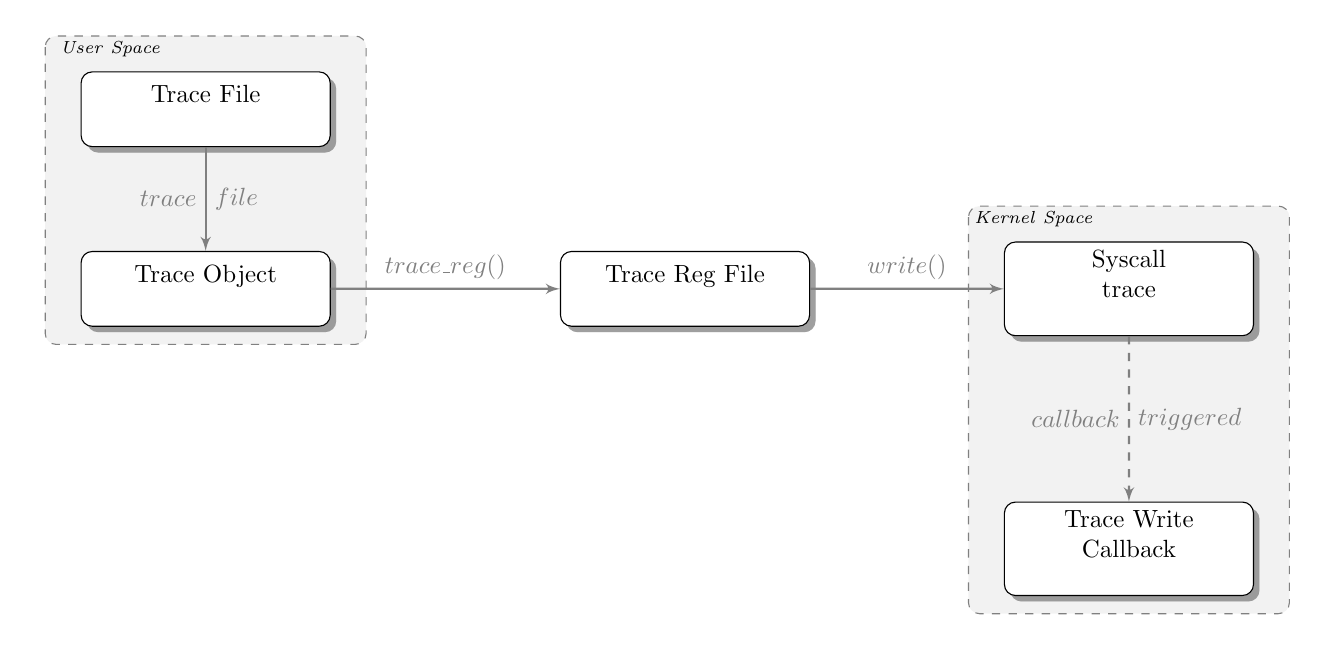
\begin{tikzpicture}[scale=0.9,transform shape]
 
  % Draw diagram elements
  % trace registration area
  \path \spacelayer {TRACEFILE}{Trace File}{};  
  \path (TRACEFILE.south)+(0.0,-2.0)\spacelayer {TRACEOBJ}{Trace Object}{};  
  \path (TRACEOBJ.east)+(5.0,0.0) \spacelayer {TRACEPROCFS}{Trace Reg File}{};
  \path (TRACEPROCFS.east)+(4.5,0.0) \spacelayer {TRACESYSCALL}{Syscall\\ trace}{};  
  \path (TRACESYSCALL.south)+(0.0,-3.0) \spacelayer {TRACECALLBACK}{Trace Write Callback}{};
  
  % Draw arrows between elements

  %thread registration block
  \path [line] (TRACEFILE.south) -- node [left] {$trace$}
									 node [right] {$file$} (TRACEOBJ);
  \path [line] (TRACEOBJ.east) -- node [above] {$trace\_reg()$} (TRACEPROCFS);

  \path [line] (TRACEPROCFS.east) -- node [above] {$write()$} (TRACESYSCALL);
  
  \path [linepart] (TRACESYSCALL.south) -- node [left] {$callback$}
                                 node [right]{$triggered$} (TRACECALLBACK);  
  
  %background generation block
  \background{TRACEFILE}{TRACEFILE}{TRACEOBJ}{TRACEOBJ}{User Space}
  \background{TRACESYSCALL}{TRACESYSCALL}{TRACECALLBACK}{TRACECALLBACK}{Kernel Space}

\end{tikzpicture}
\caption{Trace Registration}
\label{trace_reg}
\end{figure}
The trace file is passed on as an input for the scheduler. 
In figure~\ref{trace_reg}, the trace file is read by the main user thread at the start of its execution. 
It parses the file, creates and passes the trace object to the kernel space as string via a custom file created in the proc file system. 
Trace registration is implemented within the trace control module. 
The trace control module deals with the manipulation of trace object in the kernel space. 
Trace control module is imported into the scheduler module for obtaining the trace control functionality and also to access the trace itself. 
\subsection{Thread Registration}

\begin{figure}[h]
\centering
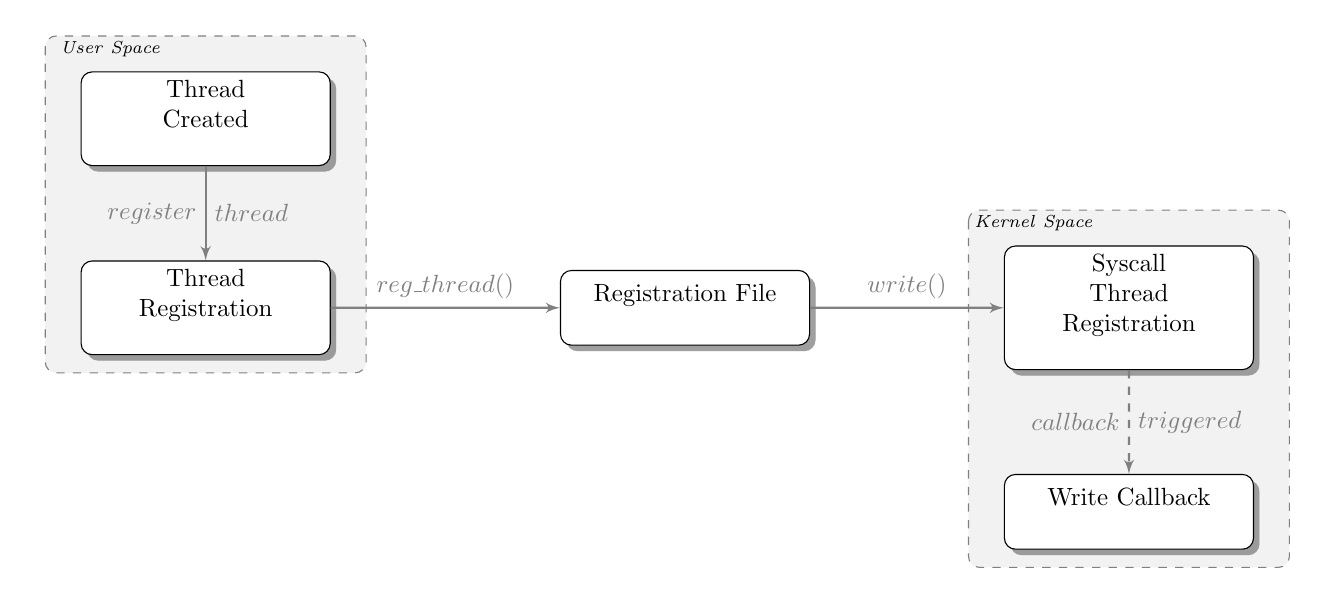
\begin{tikzpicture}[scale=0.9,transform shape] 
  
  % thread registration block area
  \path \spacelayer {THREADINIT}{Thread\\ Created}{};  
  \path (THREADINIT.south)+(0.0,-2.0)\spacelayer {USERTHREADREG}{Thread\\ Registration}{};  
  \path (USERTHREADREG.east)+(5.0,0.0) \spacelayer {REGPROCFS}{Registration File}{};
  \path (REGPROCFS.east)+(4.5,0.0) \spacelayer {REGSYSCALL}{Syscall\\ Thread\\ Registration}{};
  \path (REGSYSCALL.south)+(0.0,-2.0) \spacelayer {REGCALLBACK}{Write Callback}{};

  \background{THREADINIT}{THREADINIT}{USERTHREADREG}{USERTHREADREG}{User Space}
  \background{REGSYSCALL}{REGSYSCALL}{REGCALLBACK}{REGCALLBACK}{Kernel Space}
  
   %Draw arrows between elements
   %thread registration block
  \path [line] (THREADINIT.south) -- node [left] {$register$}
									 node [right] {$thread$} (USERTHREADREG);
  \path [line] (USERTHREADREG.east) -- node [above] {$reg\_thread()$} (REGPROCFS);

  \path [line] (REGPROCFS.east) -- node [above] {$write()$} (REGSYSCALL);
  
  \path [linepart] (REGSYSCALL.south) -- node [left] {$callback$}
                                 node [right]{$triggered$} (REGCALLBACK);

\end{tikzpicture}
\caption{Thread Registration}
\label{thread_reg}
\end{figure}
In figure~\ref{thread_reg}, the registration block happens when a user thread is created. 
The registration happens via a custom proc file system. 
For convenience a $thread\_reg()$ method is invoked in the user space, which internally registers the thread to the kernel space. 
The thread registration implementation is done entirely in thread registration kernel module. 
This registration is used to allocate memory space for bookkeeping the thread entry in scheduler. 
\newpage
\begin{lstlisting}[mathescape=true,style=customc,caption={Pseudo Code for checking memory access permission},frame=tlrb,label={lst:check_perm}]
mem_access = {allowed, restricted};
check_mem_acc_perm(curr_vec_clk, traceobj, thread_id tid) {
	if(clock[tid] is same in traceobj and curr_vec_clk) {
		$\forall$thread_id i in {{1...N}-{tid}}:
		if clock[i] in traceobj is greater to the one in curr_vec_clk) {
			return restricted;		
		}	
	}
	else if(clock[tid] in traceobj is lower than one curr_vec_clk) {
		return restricted;	
	}
	return allowed;
}
\end{lstlisting}


\subsection{IOCTL Manager}

\begin{figure}[h]
\centering
\begin{tikzpicture}[scale=0.7, node distance=2cm]
%Custom blocks
\node (ioctlmgr) [custblock] {IOCTL Manager};
\node (ctxtswitch) [custblock,right of=ioctlmgr,xshift =10cm,yshift =3cm] {Context Switch};
\node (signalothers) [custblock,right of=ioctlmgr,xshift =10cm,yshift =1.5cm] {Signal Other Threads};
\node (setclk) [custblock,right of=ioctlmgr,xshift =10cm] {Set Current Vector Clock};
\node (getclk) [custblock,right of=ioctlmgr,xshift =10cm,yshift =-1.5cm] {Get Current Vector Clock};
\node (resetclk) [custblock,right of=ioctlmgr,xshift =10cm,yshift =-3cm] {Reset Current Vector Clock};


%Arrows
\draw [->,thick] (ioctlmgr.east) -- (ctxtswitch);
\draw [->,thick] (ioctlmgr.east) -- (signalothers);
\draw [->,thick] (ioctlmgr.east) -- (setclk);
\draw [->,thick] (ioctlmgr.east) -- (getclk);
\draw [->,thick] (ioctlmgr.east) -- (resetclk);
\end{tikzpicture}
\caption{IOCTL Manager}
\label{ioctl_mgr}
\end{figure}
IOCTL Manager is an abstraction layer in the kernel space used to contain any commands triggered from the user space. 
The manager acts as an interface for the commands requested by user space for kernel level services. 
It provides five different commands of operation as shown in figure~\ref{ioctl_mgr}. 
Among the five operations, three operations deal with the vector clock manipulation. 
The commands $context\_switch$ and $signal\_other\_threads$ are generally very expensive commands when invoked. 
You can observe their implementation in later sections of this chapter. 
$context\_switch$ command is used by all prototypes when there is a need to yield to the scheduler. 
$signal\_other\_threads$ command is used by  prototypes 1 and 3, the threads signal among themselves. 
In case of prototypes other than 1 and 3, $set\_clk$ command is used more frequent for updating a given thread's memory event. 
Updating the vector clock is a short operation when compared to signaling other threads. 
The prototypes 1 and 3 are expected showcase poor performance when encountered with the condition: $num\_memory\_constraints << total\_memory\_events$. 
These prototypes invoke $signal\_other\_threads$ command for every shared memory event thus, having a poor performance. 
Reset vector clock is invoked at the completion of the user program for resetting the clock and using it for the next execution. 
Get current vector clock is used to obtain the entire vector clock during the time of invocation. 
This command is primarily used for debugging purposes. 


\subsection{Design with no checking in user space \label{nocheck}}

In the following designs, we address the use of check for memory access  permission method entirely in kernel space. 
The pseudo implementation for the checking for memory access permission is depicted in listing~\ref{lst:check_perm}. 
All the prototypes in this thesis would be using the implementation shown in listing~\ref{lst:check_perm} for checking the memory access permission.

\subsubsection{Design with no additional scheduler thread} \label{no_check_no_add}

The design described in this section addresses the use of no additional scheduler thread. 
Prior to any global memory access, the given design would invoke IOCTL command with $context\_switch$ and thread id of the thread which addressed the memory event as its parameters. 
Prototypes 1 and 3 primarily works with a similar implementation. 
These prototypes defer in place of blocking and unblocking of the threads. 
Listing~\ref{lst:proto1} depicts the pseudo implementation of prototype 1.

\begin{lstlisting}[mathescape=true,caption={Pseudo Code for Prototype 1}, style=customc,frame=tlrb,label={lst:proto1}]
User Space:
Thread j($j \in 1..N$):
BeforeMA() {	
	ioctl(CONTEXT_SWITCH, thread_id);	
}

AfterMA() {	
	ioctl(SIGNAL_OTHER_THREADS, thread_id);
}

Kernel Space:
semaphore threads_sem[1..N] = {0...0};
Queue waitqueue={}
ctxt_switch_thread(thread_id tid) {	
	if(check_perm(tid)==restricted) {
		signal_all_other_threads(tid);
		waitqueue.push(tid);
		down(threads_sem[tid]); 
	}
}
signal_all_other_threads(thread_id tid) {
	$\forall$ thread_id i in {{1...N}-{tid}}:
		if(i in waitqueue and check_perm(i)==allowed) {
			waitqueue.remove(i);
			up(threads_sem[i]);
		}
}

\end{lstlisting}

\subsubsection{Design with an additional scheduler thread}\label{sec_add_thread}

In this design, we have an additional scheduler thread which addresses the signaling mechanism pertained in the previous design. 
By having an additional scheduler thread, we move the entire signaling system to the scheduler thread.
Thus, reducing the execution overhead encountered in the pool of user space threads for signaling other threads.
The major changes are in kernel space code. 
However, there are minor variations in the $AfterMA()$ in user space. 
Inside the $AfterMA()$ call, we invoke the $set\_clk$ command. 
It is used to update the memory event for the thread which encountered the memory event. 
Prototypes 2 and 4 follow similar implementation. 
However, they defer in the blocking and unblocking mechanism of the thread. 
\begin{lstlisting}[mathescape=true,caption={Pseudo Code for Prototype 2}, style=customc,frame=tlrb,label={lst:proto2}]
User Space:
Thread j($j \in 1..N$):
BeforeMA() {	
	ioctl(CONTEXT_SWITCH, thread_id);	
}

AfterMA() {	
	ioctl(SET_CLK, thread_id);
}

Kernel Space:
semaphore threads_sem[1..N] = {0...0};
Queue waitqueue={};

Run a kernel level thread every 1ms which invokes signal_permitted_threads function.

ctxt_switch_thread(thread_id tid) {	
	if(check_perm(tid)==restricted) {
		waitqueue.push(tid);
		down(threads_sem[tid]); 
	}
}
set_clk(thread_id tid) {
	vec_clk[tid]++;
}
signal_permitted_threads() {
	$\forall$ thread_id i in {1...N}:
		if(i in waitqueue and check_perm(i)==allowed) {
			waitqueue.remove(i);
			up(threads_sem[i]);
		}
}
\end{lstlisting}

\subsection{Design with proxy checking in user space\label{proxycheck}}

In the following designs, we address the use of checking for memory access permission both in user space and kernel space.

\subsubsection{Design with no additional scheduler thread}

Without an additional thread in kernel space, the design would require a signaling function inside $AfterMA()$, similar to the one used in Design~\ref{no_check_no_add} with no additional scheduler thread. 
Triggering a signaling mechanism is an additional overhead on the thread calling the $AfterMA()$. 
Therefore, such a design is not a wise choice when considering the performance metrics such as execution time.
 
\subsubsection{Design with an additional scheduler thread}

The scheduler implementation is similar to one defined in the section \ref{sec_add_thread} with an additional scheduler thread. 
Key difference is the additional checking for memory access permissions in the user space. 
The major changes are in user space code. 
Prototypes 5 and 6 use a similar setup as shown in listing~\ref{lst:proto5}. 
However, they differ in their blocking and unblocking mechanism of threads. 
As explained in the previous sections, this design is expected to perform better under the following condition: $num\_memory\_constraints << total\_memory\_events$. 

\begin{lstlisting}[mathescape=true,caption={Pseudo Code for Prototype 5 and 6}, style=customc,frame=tlrb,label={lst:proto5}]
User Space:
Thread j($j \in 1..N$):
BeforeMA() {	
	if(check_perm(j)==restricted) {
		ioctl(CONTEXT_SWITCH, thread_id);	
	}
}

AfterMA() {	
	ioctl(SET_CLK, thread_id);
}
//Rest of the code remains the same.
\end{lstlisting}
\subsection{Variant in blocking implementation}

In the previous designs, the blocking was done using semaphores. 
In the variant design, we use the combination of $schedule()$ and $wake\_up\_process()$ functions provided by the Linux scheduler APIs. 
The kernel level tasks associated for the provided user level threads are moved from running queue to wait queue by initially setting the task status as $TASK\_INTERRUPTIBLE$ and yielding the processor by invoking $schedule()$. 
The task added in wait queue is later resumed, when $wake\_up\_process(sleeping\_task)$ is invoked by another task(primarily another thread). 
On calling the $wake\_up\_process(sleeping\_task)$, the task status for $sleeping\_task$ is set as $TASK\_RUNNING$. 
It would be pushed to run queue and executed in future by the operating system scheduler on the basis of scheduler class and priority of tasks in run queue. 
Prototype 3,4 and 6 utilizes this design.
Listing~\ref{lst:proto3} and \ref{lst:proto4} depicts Prototypes 3 and 4.  

\begin{lstlisting}[mathescape=true,caption={Pseudo Code for Prototype 3}, style=customc,frame=tlrb,label={lst:proto3}]
//rest remains the same.
Kernel Space:
Queue waitqueue={}
ctxt_switch_thread(thread_id tid) {	
	if(check_perm(tid)==restricted) {
		signal_all_other_threads(tid);
		waitqueue.push(tid);
		set_current_task_state(TASK_WAIT);
		schedule();
	}
}
signal_all_other_threads(thread_id tid) {
	$\forall$ thread_id i in {{1...N}-{tid}}:
		if(i in waitqueue and check_perm(i)==allowed) {
			waitqueue.remove(i);
			wakeup_process(taskforthreadid(i));
		}
}
\end{lstlisting} 
\begin{lstlisting}[mathescape=true,caption={Pseudo Code for Prototype 4}, style=customc,frame=tlrb,label={lst:proto4}]
//rest remains the same.
Kernel Space:
Run a kernel level thread every 1ms which invokes signal_permitted_threads function.
Queue waitqueue={}
ctxt_switch_thread(thread_id tid) {	
	if(check_perm(tid)==restricted) {	
		waitqueue.push(tid);
		set_current_task_state(TASK_WAIT);
		schedule();
	}
}
signal_permitted_threads() {
	$\forall$ thread_id j in {1...N}:
		if(j in waitqueue and check_perm(j)==allowed) {
			waitqueue.remove(j);
			wakeup_process(taskforthreadid(j));
		}
}
//rest remains the same.
\end{lstlisting}

\subsection*{Additional Note}

We have $signal\_all\_other\_threads()$ method invoked within $ctxt\_switch\_thread()$ method in Prototypes 1 and 3. 
The above call is made from $ctxt\_switch\_thread()$ to ensure that the design does not run into any deadlocks. 

A $waitqueue$ is used in all the prototypes. 
It is used to maintain a bookkeeping for all the blocked threads. 
A design without $waitqueue$ would require the checking memory access permission with the trace to be done differently. 
The modified design would have all the signaling threads checking the trace for all threads which could be blocked and signaling all the blocked threads independently whereas, in the design discussed in this thesis we use a $waitqueue$. 
The waitqueue is implemented as an array of boolean values and with size of total number of threads. 
To check if a thread is blocked or not, we can access array with the thread's id as its index. 
Firstly, such a modified design highlights a possibility of a race conditions when removing a memory event from a trace. 
A memory event is removed from the trace once the event is completed. 
Secondly, the prototypes using semaphores(Prototypes 1,2 and 5) could not be adapted with such design changes. 
Let us consider that, there are 4 threads in the multithreaded program. 
Three of the threads are running, whereas the last thread is blocked. 
When all first three threads invoke the $signal\_other\_threads()$ method, they would perform the $up$ operation on the semaphore variable meant for last thread(assuming that the fourth thread is allowed to execute). 
Problem here is that the value of the semaphore say $sema_4$ would be 3 and not one, value 3 would indicate the fourth thread to miss the yield functionality for the next three restricted memory access. 
As indicated in the appendix~\ref{appendixc}, we use a binary semaphore and not a counting semaphore for the threads in Prototypes 1,2 and 5. 
To avoid the race conditions, we could have a mutex around the code section which deals with the removal of the memory event from the trace. 
Invoking mutexes or locks regularly can affect the performance of the multithreaded program~\citep{torrellas1994false}. 
Having a mutex inside this code section would increase the execution overhead drastically. 
Moreover, such a design with mutex would make the design  to be logically equivalent to the one with the $waitqueue$. 
Therefore, there is no gain in making such a change. 

The algorithmic time complexity for running $signal\_all\_other\_threads()$ is $O(n^2)$, whereas $set\_clk()$ is $O(1)$. 
In $ctxt\_switch\_thread()$ method we have higher algorithmic time complexity in Prototypes 1 and 3, since they invoke $signal\_all\_other\_threads()$ internally.
	
	\chapter{Evaluation \label{eval_ch}}	
	In this chapter, we perform various experiments to get a better understanding of the IRS kernel space implementations proposed in the previous chapter. 
The experiments are intended to provide a comparison between user space and kernel space IRS implementations. 
The comparison between the above implementations are evaluated across multiple processor cores ranging from two to eight cores.  
We evaluate kernel space solutions based on the number of calls made to kernel space for synchronization. 
Four benchmarking programs are used for all the above mentioned evaluations.

\section{Setup}

The evaluation is performed with a virtual machine running on a hardware with Intel Xeon E5-2650 - 2.00 GHz(16 cores) configured with Ubuntu 17.04 as the operating system. 
It is configured with 4GB RAM and 80GB hard disk. 
The virtual machine(VM) is configured with the LLVM-CLANG 3.9, GCC 4.9 and Boost 1.6.2. 
We use multiple VM configurations ranging from two cores to eight cores for various evaluations. 
Configurations by scaling the number of processor cores is mainly intended to perform a scaled evaluation of cores to number of threads across various IRS implementations for a given benchmark.

\section*{Note}

We would be using the following abbreviations in the rest of the evaluations for simplicity of expression.
\begin{itemize}
\item {IRS\_Sh} - One of the IRS user space implementation discussed in sections~\ref{iter_rel_sched} and \ref{mot}. 
It addresses the use of a busy waiting design for blocking a thread and use the other threads in the thread pool to signal the blocked thread. 
Thus, making the scheduling decision shared among the threads. 
This design does not have an additional thread for handling the scheduling decisions. 
\item {IRS\_Opt} - Another user space IRS solution discussed in sections~ \ref{iter_rel_sched} and \ref{mot}. 
It uses an additional thread for handling the scheduling decisions and uses conditional variables to block a certain thread when memory access is restricted. 
\item {Proto\_1} - Section~\ref{sync_des} highlights all the prototypes used in this thesis to provide various solutions addressing the transition of scheduling decision to kernel space. 
Prototype 1 is the first synchronization discussed in section~\ref{sync_des} which uses a shared scheduler design similar to IRS\_Sh but, the blocking of threads is enforced by using semaphores in kernel space. 
\item {Proto\_2} - Prototype 2 is an extension of the previous prototype. 
Prototype also uses semaphores in kernel space for blocking a given thread but, the signaling the blocked thread is done by an additional thread which is similar to IRS\_Opt.
\item {Proto\_3} - Prototype 3 is a lot similar to Prototype 1 in the nature of behavior when it comes to design and its approach to scheduling. 
Main difference of Prototype 3 compared to Prototype 1 is the use of scheduler APIs instead of semaphores for blocking a given thread. 
\item {Proto\_4} - Prototype 4 is a design variant of Prototype 2. It uses the same scheduling approach as Prototype 2 but, differs in the blocking of a given thread. 
It uses scheduler APIs instead of semaphores. 
\item {Proto\_5} - Prototype 5 are an extension of Prototype 2, it is one of the designs which addresses the second approach discussed in section~\ref{sec_app}. 
As discussed in section~\ref{sec_app} it uses a proxy checking of memory access permission in user space.
\item {Proto\_6} - Prototype 6 are an extension of Prototype 4, it is another design which addresses the second approach discussed in section~\ref{sec_app}. 
As discussed in section~\ref{sec_app} it uses a proxy checking of memory access permission in user space.

\end{itemize}

In short, Proto\_1, Proto\_2, Proto\_3, Proto\_4 use the first approach discussed in section~\ref{fir_app}. 
Whereas, Proto\_5 and Proto\_6 use the second approach discussed in section~\ref{sec_app}.

\section{Benchmarks}

We use four different benchmarking programs for the evaluation of this thesis. 
The bench-marking programs are:
\begin{itemize}
\item{Fibonacci} - Program runs with two threads computing the Fibonacci numbers for 25 iterations per thread.
\item{Last Zero} - \citet{abdulla2014optimal} presents this benchmark for evaluating their work. The benchmark program runs with 16 threads.
\item{Indexer}- \citet{dynamic_por} use this benchmark program for evaluation of their work. The benchmark program runs with 15 threads.
\item{Dining Philosophers Problem} - The benchmark program runs with 16 threads. 
This benchmark is motivated from the solution presented in \citet{silberschatz2014operating}.
\end{itemize}

We generate memory constraints(constraints addressing shared memory events) for the above benchmarks in the form of an execution trace stored in a trace file. 
The trace file is a graphviz representation. 
The trace file is manually generated based on the benchmark in use. 
It could be automated in the future by having an automated verifier as discussed in the section~\ref{theor_des}.
The graphviz representation is converted manually into a vector clock representation containing only the shared memory dependencies between the  threads. 
The vector clock representation is a string depicting the inter-dependencies between threads on a shared memory event. 
We use the vector clock representation for the prototypes and graphviz file for the user space IRS solutions. 
Both the representations are logically equivalent. 
More details about their representation and conversion can be found in appendix C. 

\section{Evaluation Metrics}

\subsection{Execution Overhead}

Evaluation is done between the IRS user space solutions vs kernel space solutions. 
Execution overhead is calculated for each solution with respect to the plain execution of the benchmarking program. 
Unconstrained execution of the program is considered as plain execution. 

$$Execution Overhead = (T_{constr} - T_{plain})/T_{plain} * 100$$

$T_{constr}$ is the execution time of the bench-marking program when executed with scheduling constraints. 
$T_{plain}$ is the plain execution time of the same bench-marking program. 
We expect to monitor the performance of various IRS implementations by checking this metric. 
If execution overhead for a certain IRS design is the smallest, that design is considered to give the best performance. 

\subsection{Number of necessary synchronization calls} 

This metric used to realize the number of necessary calls made to the kernel space for synchronization purposes. 
The number of synchronization calls are primarily the number of IOCTL calls made under the commands: context\_switch, signal\_all\_other\_threads or set\_clock. 
The term `necessary' is validated based on the number of IOCTL calls which actually performs the synchronization operations for the commands mentioned above. 
Whereas in case of `unnecessary' calls, we observe a behavior of IOCTL calls returned to the user space without any major influence or changes in the kernel space. 
We record the number of IOCTL calls with the command context\_switch and determine the prototypes which provide a smaller overhead. 
We expect some of the prototypes to make unnecessary calls to kernel space when requesting a context switch. 
These unnecessary calls are expected to generate more overhead on execution time. 
For multithreaded programs which have extremely less number of memory constraints compared to the total number of shared memory events is expected to yield poor performance on the prototypes which yield unnecessary calls. 
Thus, making this evaluation metric a crucial parameter when comparing various prototypes. 
More explanation about such a behavior is discussed in section~\ref{sec_app}.  
We describe the use of this metric more in this section~\ref{vol_kernel_calls}.  


\section{Number of synchronization calls \label{vol_kernel_calls}}

We evaluate the number of necessary calls made to kernel space for synchronization operation. 
The evaluation is done across all six prototypes described in this thesis. 
The benchmark used for the evaluation is Fibonacci. 
The Fibonacci benchmark presents different levels of memory constraints via its traces. 
It has three traces providing 98 constraints, 44 constraints and 24 constraints respectively. 

\begin{table}[h]
\begin{center}
 \begin{tabular}{|c c c|} 
 \hline
 & Prototype 1-4 & Prototype 5-6\\ %[0.5ex] 
 \hline
 Trace-1 & 300 & 175\\ 
 Trace-2 & 300 & 150\\
 Trace-3 & 300 & 150\\
 \hline
\end{tabular}
\end{center}
\caption{Number of IOCTL calls}
\label{num_ioctls}
\end{table}
\begin{table}
\begin{center}
 \begin{tabular}{|c c c|} 
 \hline
 & Prototype 1-4 & Prototype 5-6\\ %[0.5ex] 
 \hline
 Trace-1 & 150 & 27\\ 
 Trace-2 & 150 & 0\\
 Trace-3 & 150 & 0\\
 \hline
\end{tabular}
\end{center}
\caption{Number of context switch calls}
\label{num_ctxts}
\end{table}

From the tables~\ref{num_ioctls} and \ref{num_ctxts}, it is evident that prototypes 5 and 6 reduce the number of calls made to kernel space. 
Prototypes 5 \& 6 are expected to provide better performance compared to other prototypes, when the number of memory constraints in the trace is extremely less than the total number of shared memory events in the benchmark as depicted in equation~\ref{mem_cond}. 
Section~\ref{sec_app} provides a detailed explanation of the approach used in prototypes 5 and 6, and the reason for their better performance. 

The Fibonacci benchmark has two threads with a total of 75 shared-memory events per thread. 
Thus, making a total of 150 memory events. 
For every shared-memory event, prototypes 1-4 trigger IOCTL calls to kernel space for context\_switch, signal\_all\_other\_threads or set\_clock. 
Therefore, having a total number of IOCTL calls as 300. 
In case of prototype 5-6, we have a proxy checking for shared memory access  in user space which drastically reduces the calls to kernel space for additional synchronization. 
The set\_clock ioctl command is the only call made consistently for every memory access when using prototypes 5-6.

\begin{table}[h]
\begin{center}
 \begin{tabular}{|c c c c c c c|} 
 \hline
 & Proto-1 & Proto-2 & Proto-3 & Proto-4 & Proto-5 & Proto-6\\ %[0.5ex] 
 \hline
 Trace-1 & 406.833 & 454.785 & 385.416 & 455.745 & $277.793$ & $275.343$ \\ 
 Trace-2 & 367.199 & 520.352 & 352.506 & 509.843 & $160.266$ & $160.307$ \\
 Trace-3 & 351.029 & 416.653 & 333.704 & 412.206 & $152.425$ & $153.06$\\
 \hline
\end{tabular}
\end{center}
\caption{Execution overhead(\%) when compared with plain execution of Fibonacci across six prototypes}
\label{fib_exec_over}
\end{table}

Table~\ref{fib_exec_over} shows us that the execution overhead is drastically reduced for the prototypes 5 and 6. 
Reduction in the number of IOCTL calls is reason for such a difference in the execution overhead. 
Prototypes 5-6 provide lower execution time overhead compared to other prototypes, when the condition indicated in equation~\ref{mem_cond} is satisfied. 

\section{Comparison between user space and kernel space IRS solutions}

In this evaluation, we understand the merits and demerits in the performance of the six prototypes and the two user space IRS implementations. 
For this evaluation, we use four bench-marking programs - Fibonacci, Last Zero, Indexer and Dining Philosophers Problem. 
We scale the processor configuration from two to eight processor cores and monitor the changes in the performance overhead across the benchmarks - Last Zero, Indexer and Dining Philosophers Problem for the various IRS implementations. 
Fibonacci benchmark is evaluated only with the configuration of two processor cores because the number of threads configured for the benchmark is two. 
The best prototype among the six prototypes is chosen and compared with IRS user space implementation for each benchmark.
Scaling the number of cores aids in the scalability evaluation of various IRS implementations. 
Such an evaluation also helps to realize the possibility of false sharing problem in the designs. 

\subsection{Fibonacci}

\begin{figure}[h]
     \centering
     \subfloat[][User space vs Best Prototype]{\includegraphics[scale=0.5]{../../evaluations/cores_2/eval_fibonacci_best.png}\label{fibonacci_best_cores_2}}
     \subfloat[][Comparison between prototypes]{\includegraphics[scale=0.5]
{../../evaluations/cores_2/eval_fibonacci_protos.png}
\label{fibonacci_protos_cores_2}}
     \caption{Comparison of IRS with Fibonacci on two cores}
\end{figure}

Fibonacci benchmark has two threads at its disposal. 
The pseudo code of this benchmark is depicted in listing~\ref{code_fibonacci}. 
The trace files for this benchmark provides 98, 44 and 24 memory constraints. 
The memory constraints indicated in this benchmark are the shared memory dependencies between the two threads in the benchmark. 
The benchmark is configured to run for 25 iterations. 
For every iteration as seen in listing~\ref{code_fibonacci}, we have three shared memory event. 
These memory events include two consecutive reads and one final write. 
There are three memory events for iteration and there are two threads in total for this benchmark. 
Thus, having a total of 150 shared memory events. 
The execution overhead is expected to be higher when the number of memory constraints are close to total shared memory events. 
For the first trace file (98 memory constraints), we expect to have a higher execution overhead in IRS user space implementations and comparatively lower overhead in kernel space implementations. 
With the third trace(24 memory constraints), we expect the difference in the execution overhead of IRS user space solutions to the prototypes to be smaller. 
The key reason for such a behavior is that we expect the user space solutions to perform better when the number of memory constraints in the benchmarking programs are far less to the total number of shared memory events in the program. 

From figure~\ref{fibonacci_protos_cores_2}, we observe that Proto\_5 and Proto\_6 provide the best performance among all the prototypes. 
The reason for such a behavior is the condition depicted in equation~\ref{mem_cond} satisfies. 
Section~\ref{sec_app} presents a detailed reasoning for such a behavior. 
Another interesting observation is the growth rate in relation to execution overhead for Prototypes 5-6 compared to other prototypes when the number of memory constraints are increased. 
When the number of memory constraints is increased from 44 to 98, in prototypes 5-6 we observe an increase in execution overhead from 160\% to nearly 300\%. 
Whereas in case of prototypes 1 and 3, we observe only a small increase from 350\% to 380\%. 
From this behavior we can extrapolate that when the number of memory constraints in the benchmark gets closer to the total number of shared memory events, prototypes 1-4 would have comparatively low execution overhead to prototypes 5-6. 
The reason for such a behavior is explained in section~\ref{fir_app}. 

From figure~\ref{fibonacci_protos_cores_2}, we have taken Proto\_5 as best prototype for this benchmark. 
Proto\_6 provides nearly the same results but, we have chosen only one of the two. 
From figure~\ref{fibonacci_best_cores_2}, we observe a very low overhead depicted by Proto\_5 compared to the two user space solutions. 
When the number of memory constraints are reduced, we observe a decline in the execution overhead for the user space solutions. 
It is evident when number of memory constraints is reduced from 44 to 24. 
IRS\_Sh seems to provide the best performance among the two user space solutions of IRS. 
The reason for such a behavior is that there is no additional thread in IRS\_Sh and it is implemented with a busy waiting design. 
One of the benefits of busy waiting design is that it is very responsive when the number of threads are less than or equal to the number of cores. 
IRS\_Opt depicts the worse performance among all the IRS designs. 
IRS\_Opt utilizes additional thread for signaling the blocked threads. Thus, making a total of 3 threads for this program. 
For every memory event we have 3 threads running on two cores. 
The possibility of the scheduler thread(the additional thread used by IRS\_Opt for scheduling) getting context switched is higher. 
The results shown in figure~\ref{fibonacci_best_cores_2} validates the above mentioned hypothesis.


\subsection{Last Zero}

\citet{abdulla2014optimal} showcase this benchmark for the evaluation of their dynamic POR. 
The last zero program has 16 threads at its disposal. 
The pseudo code of this benchmark is depicted in listing~\ref{code_lastzero}. 
This benchmark is meant to provide memory constraints spread across different threads rather than being in two threads. 
The number of memory constraints provided in the trace files include: 15, 12, 5, 1 respectively. 
The maximum number of possible shared memory events is 46 and minimum being 31 shared memory events.

\begin{figure}[h]
     \centering
     \subfloat[][User space vs Best Prototype]{\includegraphics[scale=0.5]{../../evaluations/cores_2/eval_last_zero_best.png}\label{last_zero_best_cores_2}}
     \subfloat[][Comparison between prototypes]{\includegraphics[scale=0.5]
{../../evaluations/cores_2/eval_last_zero_protos.png}
\label{last_zero_protos_cores_2}}
     \caption{Comparison of IRS with Last Zero on two cores}
\end{figure}


\begin{figure}[h]
     \centering
     \subfloat[][User space vs Best Prototype]{\includegraphics[scale=0.5]{../../evaluations/cores_4/eval_last_zero_best.png}\label{last_zero_best_cores_4}}
     \subfloat[][Comparison between prototypes]{\includegraphics[scale=0.5]{../../evaluations/cores_4/eval_last_zero_protos.png}
\label{last_zero_protos_cores_4}}
     \caption{Comparison of IRS with Last Zero on four cores}
\end{figure}


\begin{figure}[h]
     \centering
     \subfloat[][User space vs Best Prototype]{\includegraphics[scale=0.5]{../../evaluations/cores_8/eval_last_zero_best.png}\label{last_zero_best_cores_8}}
     \subfloat[][Comparison between prototypes]{\includegraphics[scale=0.5]{../../evaluations/cores_8/eval_last_zero_protos.png}
\label{last_zero_protos_cores_8}}
     \caption{Comparison of IRS with Last Zero on eight cores}
\end{figure}

This benchmark has 16 threads in total. 
In the first trace file(15 memory constraints), we have atleast one dependency for each thread except for the first thread(thread with id as 0). 
The first trace provides some diversity in the number of memory constraints realized with this benchmark. 
With the evaluation configured for two, four and eight processor cores, we expect the IRS\_Sh to provide the worst performance of the all IRS implementations. 
IRS\_Sh is a busy waiting design. 
Busy waiting design makes the waiting thread to constantly poll one of the cores thus, making it performance inefficient. 
This benchmark has dependencies across all 16 threads with the first trace file and there are more number of threads to the number of processor cores, thus making the busy waiting design to perform poorly among all the other designs for the first trace. 
However, it is expected to improve the execution overhead with the scaling of cores. 
The condition depicted in equation~\ref{mem_cond} satisfies in this benchmark for all the traces thus, making prototypes 5 and 6 to provide the best performance among all the prototypes. 
Section~\ref{fir_app} highlights this condition in more detail manner.  


The results depicted in figures~\ref{last_zero_protos_cores_2}, \ref{last_zero_protos_cores_4}, \ref{last_zero_protos_cores_8} show us that Proto\_1 and Proto\_3 performs better for first trace(number of memory constraints are 15) because the number of memory constraints are closer to the total shared memory events in the benchmarking program. 
From Fig~\ref{last_zero_protos_cores_2}, it is evident that Proto\_5 and Proto\_6 performs nearly the same when it comes to execution overhead. 
For traces which have less number of memory constraints(traces 3, 4 have 5, 1 constraints respectively), Proto\_5 and Proto\_6 performs better among all prototypes in overall. 
From Figures~\ref{last_zero_best_cores_2}, \ref{last_zero_best_cores_4}, \ref{last_zero_best_cores_8}, it is evident that IRS\_Sh performs the worst for this benchmark compared to all the other IRS implementations. 
From Figures~{\ref{last_zero_best_cores_2}, \ref{last_zero_best_cores_4}, \ref{last_zero_best_cores_8}, we observe that execution overhead for IRS\_Sh reduces with the increase in the number of cores. 
From these results, we can extrapolate that the execution overhead would be much lower for IRS\_Sh if the number of processor cores were 16 or more. 
As explained in the previous paragraph, it is because IRS\_Sh is based on a busy waiting design. 
IRS\_Opt provides the best performance among all the IRS solutions under all evaluations of this benchmark. 
It performs better than IRS\_Sh because it uses a condition variable design with an additional thread for handling the scheduling decisions. 
Based on the results for this benchmark, we can conclude that the overhead generated by the pthread library on the IRS\_Opt would be less compared to all the other IRS designs. 
Thus, making IRS\_Opt best choice among all the IRS designs for benchmarks which follow similar conditions and configurations to this benchmark. 




%----------------------------------------------------------------------------
\subsection{Indexer}



%Evaluation of indexer with cores-------
\begin{figure}[h]
     \centering
     \subfloat[][User space vs Best Prototype]{\includegraphics[scale=0.5]{../../evaluations/cores_2/eval_indexer_best.png}\label{indexer_best_cores_2}}
     \subfloat[][Comparison between prototypes]{\includegraphics[scale=0.5]{../../evaluations/cores_2/eval_indexer_protos.png}\label{indexer_protos_cores_2}}
     \caption{Comparison of IRS with Indexer on two cores}
\end{figure}


\begin{figure}[h]
     \centering
     \subfloat[][User space vs Best Prototype]{\includegraphics[scale=0.5]{../../evaluations/cores_4/eval_indexer_best.png}\label{indexer_best_cores_4}}
     \subfloat[][Comparison between prototypes]{\includegraphics[scale=0.5]{../../evaluations/cores_4/eval_indexer_protos.png}\label{indexer_protos_cores_4}}
     \caption{Comparison of IRS with Indexer on four cores}
\end{figure}


\begin{figure}[h]
     \centering
     \subfloat[][User space vs Best Prototype]{\includegraphics[scale=0.5]{../../evaluations/cores_8/eval_indexer_best.png}\label{indexer_best_cores_8}}
     \subfloat[][Comparison between prototypes]{\includegraphics[scale=0.5]{../../evaluations/cores_8/eval_indexer_protos.png}\label{indexer_protos_cores_8}}
     \caption{Comparison of IRS with Indexer on eight cores}
\end{figure}

\citet{dynamic_por} utilize this benchmark for evaluating their dynamic POR design. 
The pseudo code for the indexer program is realized in listing~\ref{code_indexer}.  
The indexer program revolves around a hash table, where threads read and write hashed messages on it. 
Each thread calculates four messages and writes them to a shared hash table. 
Collisions are detected and avoided using the compare and swap(cas) statement. 
The message values depend on the thread id. 

For our experiments, we have used 15 threads with the indexer program. 
The benchmark contains approximately 60 shared-memory events in total. 
Six traces are used with the following as the number of memory constraints: 12, 8, 4, 3, 2, 1. 
The memory constraints are set in a way that all the constraints are within a span of four threads and not all 15 threads. 
For the first trace, we have three memory constraints in each of the four threads.
We expect to have good performance for IRS\_Sh because the number of constraints are not spread across all 15 threads. 
We expect it to perform the best when the core count is 8, even when the number of constraints are set at 12. 
Proto\_5 and Proto\_6 are expected perform best among all the prototypes for this benchmark, because the condition indicated in equation~\ref{mem_cond} satisfies. 

From figures~\ref{indexer_protos_cores_2}, \ref{indexer_protos_cores_4}, \ref{indexer_protos_cores_8}, it is evident that Proto\_5 and Proto\_6 performs the best among the prototypes in all scenarios for this benchmark. 
Based on the analysis of figures~\ref{indexer_best_cores_2}, \ref{indexer_best_cores_4}, \ref{indexer_best_cores_8}\, we observe a trend in the improvement of execution overhead in IRS\_Sh. 
As expected IRS\_Sh provides the best performance when the number of cores is eight as observed in Figure~\ref{indexer_best_cores_8}.
However, IRS\_Opt showcases a huge overhead for this benchmark. 
One of the reasons for such a poor performance would be the lack of diversity of memory constraints(diversity indicates that the memory constraints are within a span of four threads not all 15 threads). 
There are few anomalies in the results, such as the increase in execution overhead for IRS\_Opt when number of memory constraints is 1 as shown in figure~\ref{indexer_best_cores_4}. 
There is no theoretical explanation for such an increase. 
Another anomaly is when the number of memory constraints is 3 and the configuration for processor count is set to two as shown in figures~\ref{indexer_protos_cores_2} and \ref{indexer_best_cores_2}, we observe an increase in execution overhead for all designs except IRS\_Opt. 
The trace file with three memory constraints spans three threads. 
Thus, making a one thread sleep longer in such a scenario eventually creating a surge in execution overhead. 




%----------------------------------------------------------------------------
\subsection{Dining Philosopher's Problem}

%Evaluation of Dining Phil with cores-------
\begin{figure}[h]
     \centering
     \subfloat[][User space vs Best Prototype]{\includegraphics[scale=0.5]{../../evaluations/cores_2/eval_dining_phil_best.png}\label{dining_phil_best_cores_2}}
     \subfloat[][Comparison between prototypes]{\includegraphics[scale=0.5]{../../evaluations/cores_2/eval_dining_phil_protos.png}\label{dining_phil_protos_cores_2}}
     \caption{Comparison of IRS with Dining Philosophers Problem on two cores}
\end{figure}

\begin{figure}[h]
     \centering
     \subfloat[][User space vs Best Prototype]{\includegraphics[scale=0.5]{../../evaluations/cores_4/eval_dining_phil_best.png}\label{dining_phil_best_cores_4}}
     \subfloat[][Comparison between prototypes]{\includegraphics[scale=0.5]{../../evaluations/cores_4/eval_dining_phil_protos.png}\label{dining_phil_protos_cores_4}}
     \caption{Comparison of IRS with Dining Philosophers Problem on four cores}
\end{figure}

\begin{figure}[h]
     \centering
     \subfloat[][User space vs Best Prototype]{\includegraphics[scale=0.5]{../../evaluations/cores_8/eval_dining_phil_best.png}\label{dining_phil_best_cores_8}}
     \subfloat[][Comparison between prototypes]{\includegraphics[scale=0.5]{../../evaluations/cores_8/eval_dining_phil_protos.png}\label{dining_phil_protos_cores_8}}
     \caption{Comparison of IRS with Dining Philosophers Problem on eight cores}
\end{figure}

The Dining Philosopher's Problem is a well known synchronization problem in the domain of concurrency problems. 
There are many solutions adhered to overcome the problem. 
\citet{silberschatz2014operating} have addressed many solutions in their book for the above problem. 
We are using one of the solutions proposed in their book. 
The solution uses two classes of philosophers - odd and even philosopher. 
The classification is based on the thread id of the philosopher threads. 
Every odd philosopher checks the chopstick on the left before checking on the right for availability. 
The opposite in case of even philosopher. 
The solution for this problem is showcased in listing~\ref{code_dining_phil}.

In our experiments, we have adapted the solution to have 16 threads and 10 iterations. 
Compared to previous benchmarks which had only few constraints, this benchmark has more constraints and spans across all 16 threads. 
This benchmark is expected to run in milliseconds time range rather than microseconds which was evident with respect to the previous benchmarks. 
For getting a detailed understanding of the experimental results, please refer to appendix~\ref{appendixb}.  

This benchmark has 16 threads at its disposal. 
There are nearly 60 shared-memory events per thread. 
Thus, making a total of 960 shared-memory events in total. 
The benchmark has at-most eight threads running at any point of time. 
The number of memory constraints listed for the three traces include: 56, 24, 8. 
The first trace contains memory constraints spanning all the threads.
This benchmark satisfies the condition depicted in equation~\ref{mem_cond} in all trace file conditions. 
Prototype 1-4 follow the first approach discussed in section~\ref{fir_app}. 
Evaluation on the number of necessary synchronization calls highlighted in section~\ref{vol_kernel_calls}, infers that the prototypes 1-4 to perform poorly when the condition mentioned in equation~\ref{mem_cond} satisfies. 
Among prototypes 1-4, we expect prototype 1 and 3 to perform the worst under these conditions. 
Proto\_1 and Proto\_3 are kernel space solutions implemented with a shared scheduler in place. 
Proto\_1 and Proto\_3, performs $signal\_other\_threads$ call from $AfterMA()$ of every shared memory event. 
As depicted in section~\ref{nocheck}, signaling of other threads is a costly operation compared to updating a vector clock(prototypes 2 and 4 updates vector clock instead of signaling threads). 
Thus, making Proto\_1 and Proto\_3 to perform the worst among the prototypes. 
We expect Proto\_5 and Proto\_6 to provide the best performance among the prototypes because of the condition mentioned in equation~\ref{mem_cond}.
IRS\_Sh is expected to give away a very poor performance because of the diversity of constraints and since it is based on busy waiting design.  

From figures~\ref{dining_phil_protos_cores_2}, \ref{dining_phil_protos_cores_4}, \ref{dining_phil_protos_cores_8}, it is evident that Proto\_5 and Proto\_6 perform the best among the prototypes under all the scenarios of this benchmark. 
Proto\_1 and Proto\_3 as expected came up with the worst performance among the prototypes. 
In case of the comparison with the user space implementation, IRS\_Opt seems to have the smaller overhead compared to IRS\_Sh. 
From Figs~\{\ref{dining_phil_best_cores_2}, \ref{dining_phil_best_cores_4}, \ref{dining_phil_best_cores_8}\}, it is evident that IRS\_Sh seems to have the worst performance for this benchmark because of its busy waiting design. 
However, with the increase in the number for processor cores we can observe a reduction in the execution overhead for IRS\_Sh. 

\subsection{Inference on the scaling of processor cores}

The experiments performed by scaling the processor cores provided valuable insight into the design problems existent in the IRS implementations.  
From the results of benchmarks- Last Zero, Indexer, Dining Philosophers Problem, it is evident that the prototypes do not scale well when the number of cores are increased.
This situation is evident with the first trace(first trace contains the highest number of memory constraints among all the traces for a given benchmark) of each benchmark as depicted in all the results. 
In kernel space for all prototypes, we have implemented vector clocks as a C struct containing an array of integer. 
Such a design was meant to provide good readability and also better memory referencing when invoked from different function. 
However, such a design drastically suffers from the problem of false sharing. 
For getting a better understanding of false sharing please refer to appendix~\ref{appendixc}.
Such an impact is clearly evident with the scaling of processor cores on the results of all three benchmarks.

\section{Inference}

The Fibonacci benchmark helped us in understanding the behavior of prototypes. 
The experiments by scaling the processor cores clearly explained the merits and demerits of various IRS designs. 
All the experiments show that Proto\_5 and Proto\_6 seem to perform the best among the prototypes in nearly all the scenarios given in the bench-marking programs. 
IRS\_Sh implementation seems to give away the worst performance in nearly all benchmarks. 
From the experiments, it is evident that all prototypes suffer from the problem of scalability. 
The IRS user space implementations performs better than the IRS kernel space implementations, when the number of memory constraints are in single digits and the number of memory constraints are comparably large. 
 
By observing the above results we can conclude that there is a need of a solution which is the combination of IRS\_Opt and Prototypes 5-6. 
This implementation would have a loadable kernel module similar to Proto\_5 or Proto\_6 however, without any checking for memory permissions in kernel space for the threads. 
The kernel module would help in providing as a forced yield of the processor to the OS Scheduler from the thread and also an interface to revive the thread. 
The check for memory access permission would be implemented entirely in the user space and calls would be made to the above mentioned kernel space solution for yielding the processor.  
In short, this kernel space interface would be used instead of using condition variables in IRS\_Opt.

	
	\chapter{Conclusion}
	The IRS scheduler designs implemented in this thesis highlights a new approach in designing the scheduler for the IRS framework which involved by  moving the scheduler logic to kernel space. 
We introduced two different design approaches in moving the IRS scheduler to kernel space. 
The first approach triggers an IOCTL call to kernel space for every shared memory event.
In the second approach, we reduce the number of IOCTL calls made to the kernel space for every shared memory event. 
The reduction in the number of IOCTL calls is achieved by having a proxy checking for memory access permission during a shared memory event. 
The kernel space solutions presented with six different prototypes. 
The first four prototypes used the first approach and the last two prototypes were realized with the second approach. 
All the prototypes presented in this thesis were incremental improvements over its former.
We also introduced an alternative representation in the form of vector clocks for realizing the scheduling constraints enforced on threads in a multithreaded program. 
The vector clock representation was intended to reduce the code complexity and for overcoming one of the design challenges of this thesis. 

In our experiments, we compared the IRS user space and IRS kernel space solutions with the benchmarking programs - Fibonacci, Last Zero, Indexer and Dining Philosopher's Problem. 
In our experiments, we observed that IRS\_Sh performed poorly when the number of threads were more than the number of cores and when the memory constraints spanned all the threads in the benchmarking program. 
We also observed that the IRS\_Opt performed better in nearly all the benchmarks but, performed poorly when the memory constraints were spanned to fewer number of threads as observed with Indexer and Fibonacci experiments. 
Among the kernel space designs, prototypes 5 and 6 performed the best in nearly all the experiments. 
However, the experiments showed us that when the number of memory constraints came closer to the total number of shared memory events Prototypes 1 and 3 were better as it can be observed with Fibonacci and Last Zero benchmarks. 
In our experiments, we observed that kernel space designs perform better when number of memory constraints are higher and closer to the total number of shared memory events. 
However, the prototypes depicted in this thesis suffer from scalability problems as observed with the experiments done on scaling of the processor cores. 
The prototypes could be optimized by removing the C-structure representation of vector clock, which could help in overcoming a potential false sharing problem. 

An experimental study of all these prototypes suggested a new design outlook for moving the IRS scheduler to kernel space. 
Based on a preliminary analysis, it is evident that there is a need of solution which is a combination of IRS\_Opt and Prototypes 5-6. 
Such a design would require the custom yield and revive functionality from prototypes 5-6 and checking for memory access permission would be handled in the user space entirely. 
In short, the condition variable design used in IRS\_Opt would be replaced by the custom yield and revive functionality from Prototypes 5-6. 
Such an approach may help to further improve the performance of constrained execution of a multithreaded program on IRS environment.


	%\input{content2}
	
	%======================================================
	% The back matter
	%======================================================
	%\cleardoublepage
	\refstepcounter{dummy}
	\addcontentsline{toc}{chapter}{\bibname}
	%\bibliographystyle{alpha} % <--- layout of the bib

	\bibliographystyle{plainnat}
	\bibliography{bibl_2} % file name of your bib

	\newpage
	%\appendix
	\begin{appendices}
	\chapter{Benchmarks}
	\section{Last Zero}
\begin{lstlisting}[mathescape=true,style=customc,caption={Last Zero Program based on \citet{abdulla2014optimal}},label={code_lastzero}]
Variables: int arr[0...N] := {0,0..,0}, i;
Thread 0: for (i:=N; array[i]!=0; i--);
Thread j($j \in 1..N$): arr[j] := arr[j-1] + 1;
\end{lstlisting}

\section{Indexer}
\begin{lstlisting}[style=customc,caption={Indexer Program based on \citet{dynamic_por}},label={code_indexer}]
Thread-global (shared) variables:
const int size = 128;
const int max = 4;
int[size] table;

Thread-local variables:
int m = 0, w, h;

Code For thread tid:
while (true) {
	w := getmsg();
	h := hash(w);
	while (cas(table[h],0,w) == false) {
		h := (h+1) % size;
	}
}
int getmsg() {
	if (m < max ) {
		return (++m) * 11 + tid;
	} else {
		exit(); // terminate
	}
}
int hash(int w) {
	return (w * 7) % size;
}
\end{lstlisting}
\newpage
\section{Dining Philosopher's Problem}

\begin{lstlisting}[style=customc,caption={Dining Philosopher's Problem Program},label={code_dining_phil}]
Thread-global (shared) variables:
const int size = THREAD_COUNT;
const int num_iter = N;
int[size] chopsticks;

Thread-local variables:
int i;

Code For thread id:
for(i=0; i<num_iter; i++) {
	while((chopsticks[id%THREAD_COUNT]!=0) && \\
	 (chopsticks[(id-1)%THREAD_COUNT]!=0);
	if(id%2==0) {
		chopsticks[id%THREAD_COUNT] = 1;
		chopsticks[(id-1)%THREAD_COUNT] = 1;
	}
	else {
		chopsticks[(id-1)%THREAD_COUNT] = 1;
		chopsticks[id%THREAD_COUNT] = 1;
	}
	chopsticks[id%THREAD_COUNT] = 0;
	chopsticks[(id-1)%THREAD_COUNT] = 0;
}
\end{lstlisting}

\section{Fibonacci}
\begin{lstlisting}[mathescape=true,style=customc,caption={Fibonacci Program},label={code_fibonacci}]
Shared Variables: int i=1,j=1;
Local Variables: int k, num_iter=N;
Thread 0: 
for (k:=0; k<num_iter; k++) {
	i+=j;
}		
Thread 1:
for (k:=0; k<num_iter; k++) {
	j+=i;
}		
\end{lstlisting}	
	\chapter{Experimental Results \label{appendixb}}
	\section{Last Zero}

\subsection{Two Cores}
\begin{table}[h]
\begin{center}
 \begin{tabular}{|c c c c c c c c c|} 
 \hline
 & IRS\_Sh & IRS\_Opt& Proto-1 & Proto-2 & Proto-3 & Proto-4 & Proto-5 & Proto-6\\ %[0.5ex] 
 \hline
Trace-1 & 3183.115 & 168.069 & 297.304 & 373.623 & 308.218 & 325.577 & 313.979 & 313.569\\
Trace-2 & 1472.212 & 119.385 & 180.815 & 230.234 & 196.77 & 204.881 & 190.245 & 190.703\\
Trace-3 & 1335.806 & 117.766 & 172.643 & 224.606 & 172.096 & 194.399 & 159.221 & 166.818\\
Trace-4 & 2.373 & 59.937 & 181.197 & 226.441 & 197.909 & 201.305 & 174.226 & 176.522\\
\hline
\end{tabular}
\end{center}
\caption{Execution overhead(\%) when compared with plain execution of Last Zero}
\label{last_zero_irs_res_cores_2}
\end{table}

\subsection{Four Cores}
\begin{table}[h]
\begin{center}
 \begin{tabular}{|c c c c c c c c c|} 
 \hline
 & IRS\_Sh & IRS\_Opt& Proto-1 & Proto-2 & Proto-3 & Proto-4 & Proto-5 & Proto-6\\ %[0.5ex] 
 \hline
Trace-1 & 2485.820 & 204.205 & 371.688 & 390.946 & 288.458 & 299.136 & 352.202 & 346.665\\
Trace-2 & 1138.293 & 117.764 & 229.857 & 260.937 & 169.108 & 196.685 & 212.92 & 206.062\\
Trace-3 & 1030.858 & 95.448 & 219.563 & 243.64 & 152.027 & 193.9 & 168.338 & 164.249\\
Trace-4 & -19.370 & 62.22 & 208.598 & 243.083 & 160.428 & 191.643 & 172.793 & 166.349\\
\hline
\end{tabular}
\end{center}
\caption{Execution overhead(\%) when compared with plain execution of Last Zero}
\label{last_zero_irs_res_cores_4}
\end{table}

\subsection{Eight Cores}
\begin{table}[h]
\begin{center}
 \begin{tabular}{|c c c c c c c c c|} 
 \hline
 & IRS\_Sh & IRS\_Opt& Proto-1 & Proto-2 & Proto-3 & Proto-4 & Proto-5 & Proto-6\\ %[0.5ex] 
 \hline
Trace-1 & 779.417 & 204.205 & 385.556 & 413.958 & 409.856 & 453.227 & 457.043 & 424.486\\
Trace-2 & 483.096 & 117.764 & 222.77 & 276.71 & 234.497 & 301.796 & 276.798 & 259.555\\
Trace-3 & 553.460 & 95.448 & 207.627 & 277.427 & 209.038 & 294.96 & 207.559 & 184.733\\
Trace-4 & 36.206 & 62.22 & 204.648 & 281.475 & 216.443 & 296.927 & 218.399 & 192.43\\
\hline
\end{tabular}
\end{center}
\caption{Execution overhead(\%) when compared with plain execution of Last Zero}
\label{last_zero_irs_res_cores_8}
\end{table}

\section{Indexer}

\subsection{Two Cores}
\begin{table}[h]
\begin{center}
 \begin{tabular}{|c c c c c c c c c|} 
 \hline
 & IRS\_Sh & IRS\_Opt& Proto-1 & Proto-2 & Proto-3 & Proto-4 & Proto-5 & Proto-6\\ %[0.5ex] 
 \hline
Trace-1 & 863.217 & 1914.739 & 357.769 & 337.66 & 356.85 & 398.296 & 310.709 & 319.146\\
Trace-2 & 591.346 & 1990.388 & 228.661 & 215.401 & 225.404 & 253.299 & 208.094 & 210.911\\
Trace-3 & 549.424 & 1961.126 & 208.925 & 199.812 & 206.814 & 239.773 & 179.803 & 181.235\\
Trace-4 & 913.520 & 1835.159 & 223.274 & 219.309 & 220.361 & 258.238 & 198.842 & 201.541\\
Trace-5 & 366.838 & 1979.13 & 206.164 & 200.645 & 203.99 & 241.717 & 181.155 & 182.518\\
Trace-6 & 114.149 & 1942.555 & 219.88 & 220.863 & 217.671 & 259.263 & 202.801 & 204.868\\
\hline
\end{tabular}
\end{center}
\caption{Execution overhead(\%) when compared with plain execution of Indexer}
\label{indexer_irs_res_cores_2}
\end{table}

\subsection{Four Cores}
\begin{table}[h]
\begin{center}
 \begin{tabular}{|c c c c c c c c c|} 
 \hline
 & IRS\_Sh & IRS\_Opt& Proto-1 & Proto-2 & Proto-3 & Proto-4 & Proto-5 & Proto-6\\ %[0.5ex] 
 \hline
Trace-1 & 668.686 & 1454.444 & 416.435 & 354.394 & 413.523 & 343.415 & 367.727 & 362.178\\
Trace-2 & 654.411 & 1382.204 & 265.879 & 233.669 & 265.585 & 223.591 & 253.029 & 246.531\\
Trace-3 & 461.305 & 1331.296 & 255.422 & 232.805 & 257.612 & 221.685 & 204.7 & 204.444\\
Trace-4 & 95.79 & 1350.194 & 249.06 & 236.008 & 250.734 & 227.052 & 209.682 & 206.575\\
Trace-5 & 35.645 & 1534.044 & 240.435 & 231.331 & 239.469 & 221.838 & 203.924 & 203.073\\
Trace-6 & 32.884 & 1813.431 & 235.273 & 242.227 & 232.892 & 233.356 & 213.21 & 210.276\\
\hline
\end{tabular}
\end{center}
\caption{Execution overhead(\%) when compared with plain execution of Indexer}
\label{indexer_irs_res_cores_4}
\end{table}
\newpage
\subsection{Eight Cores}
\begin{table}[h]
\begin{center}
 \begin{tabular}{|c c c c c c c c c|} 
 \hline
 & IRS\_Sh & IRS\_Opt& Proto-1 & Proto-2 & Proto-3 & Proto-4 & Proto-5 & Proto-6\\ %[0.5ex] 
 \hline
Trace-1 & 45.890 & 1345.816 & 387.794 & 325.782 & 392.818 & 349.26 & 321.113 & 329.815\\
Trace-2 & 31.410 & 1380.798 & 232.334 & 211.399 & 237.239 & 238.239 & 211.39 & 215.601\\
Trace-3 & 31.062 & 1386.956 & 222.408 & 216.232 & 225.199 & 231.08 & 158.417 & 160.585\\
Trace-4 & 14.880 & 1341.635 & 211.633 & 221.182 & 216.122 & 233.326 & 161.897 & 167.565\\
Trace-5 & 13.408 & 1341.658 & 199.179 & 219.984 & 204.912 & 231.014 & 161.455 & 169.477\\
Trace-6 & 9.726 & 1392.006 & 194.167 & 235.813 & 194.466 & 250.578 & 166.475 & 169.62\\
\hline
\end{tabular}
\end{center}
\caption{Execution overhead(\%) when compared with plain execution of Indexer}
\label{indexer_irs_res_cores_8}
\end{table}

\section{Dining Philosopher's Problem}

\subsection{Two Cores}
\begin{table}[h]
\begin{center}
 \begin{tabular}{|c c c c c c c c c|} 
 \hline
 & IRS\_Sh & IRS\_Opt& Proto-1 & Proto-2 & Proto-3 & Proto-4 & Proto-5 & Proto-6\\ %[0.5ex] 
 \hline
Trace-1 & 36848.947 & 2562.658 & 2021.564 & 1155.722 & 1953.05 & 1289.845 & 962.768 & 1040.711\\
Trace-2 & 15456.130 & 2449.932 & 2338.214 & 1034.048 & 2246.695 & 1181.131 & 555.116 & 558.851\\
Trace-3 & 2842.118 & 588.281 & 2085.458 & 936.671 & 2012.523 & 1070.232 & 576.78 & 569.479\\
\hline
\end{tabular}
\end{center}
\caption{Execution overhead(\%) when compared with plain execution of Dining Philosophers Problem}
\label{dining_phil_irs_res_cores_2}
\end{table}


\subsection{Four Cores}
\begin{table}[h]
\begin{center}
 \begin{tabular}{|c c c c c c c c c|} 
 \hline
 & IRS\_Sh & IRS\_Opt& Proto-1 & Proto-2 & Proto-3 & Proto-4 & Proto-5 & Proto-6\\ %[0.5ex] 
 \hline
Trace-1 & 22108.586 & 2054.342 & 2597.968 & 1672.907 & 2445.464 & 1339.063 & 1827.013 & 1801.944\\
Trace-2 & 9111.364 & 1817.914 & 2596.101 & 1368.239 & 2436.708 & 1132.18 & 742.664 & 748.36\\
Trace-3 & 697.035 & 436.169 & 2549.619 & 1240.308 & 2388.429 & 1027.419 & 720.767 & 733.722\\
\hline
\end{tabular}
\end{center}
\caption{Execution overhead(\%) when compared with plain execution of Dining Philosophers Problem}
\label{dining_phil_irs_res_cores_4}
\end{table}

\newpage
\subsection{Eight Cores}
\begin{table}[h]
\begin{center}
 \begin{tabular}{|c c c c c c c c c|} 
 \hline
 & IRS\_Sh & IRS\_Opt& Proto-1 & Proto-2 & Proto-3 & Proto-4 & Proto-5 & Proto-6\\ %[0.5ex] 
 \hline
Trace-1 & 13078.157 & 1439.948 & 2307.765 & 1293.606 & 2301.262 & 1070.26 & 1538.427 & 1536.78\\
Trace-2 & 3339.345 & 976.687 & 2225.813 & 1016.723 & 2216.829 & 864.586 & 685.367 & 661.549\\
Trace-3 & 301.401 & 365.057 & 2207.008 & 966.478 & 2185.629 & 791.868 & 625.616 & 598.105\\
\hline
\end{tabular}
\end{center}
\caption{Execution overhead(\%) when compared with plain execution of Dining Philosophers Problem}
\label{dining_phil_irs_res_cores_8}
\end{table}

	\chapter{Theoretical Explanations and Building Prototypes \label{appendixc}}
	\section{Theoretical Explanations}
\subsection{Vector Clock}
\subsection{Semaphores}
\subsection{Scheduler APIs}

\section{Building Prototypes}
	\end{appendices}	

\end{document}
